\documentclass[ms,english]{stthesis}
\usepackage{lipsum}
\usepackage[color=green]{todonotes}
\usepackage{graphicx}
\usepackage{subcaption}
\usepackage{multirow}
\usepackage{booktabs}
\usepackage{epigraph}
\usepackage{cite}
\usepackage[acronym]{glossaries}
\usepackage[most]{tcolorbox}
\usepackage{hyperref}

% \usepackage[table]{xcolor}
\usepackage{float}

\usepackage{amssymb}
% \usepackage{wasysym}

\usepackage{xspace}
\usepackage{pifont}% http://ctan.org/pkg/pifont
\newcommand{\cmark}{\ding{51}}%
\newcommand{\xmark}{\ding{55}}%

\makeglossaries
% --- MOEA
\newglossaryentry{moea}{type=\acronymtype, name={MOEA}, description={Multi-objective evolutionary algorithm}, first={Multi-objective evolutionary algorithm (MOEA)}}

% --- MOO
\newglossaryentry{moo}{type=\acronymtype, name={MOO}, description={multi-objective optimization}, first={multi-objective optimization (MOO)}}

% --- EA
\newglossaryentry{ea}{type=\acronymtype, name={EA}, description={Evolutionary algorithm}, first={Evolutionary algorithm (EA)}}







\newglossaryentry{apig}{name={API},
    description={An Application Programming Interface (API) is a particular set
of rules and specifications that a software program can follow to access and
make use of the services and resources provided by another particular software
program that implements that API}}

%%% define the acronym and use the see= option
\newglossaryentry{api}{type=\acronymtype, name={API}, description={Application
Programming Interface}, first={Application
Programming Interface (API)\glsadd{apig}}, see=[Glossary:]{apig}}


% "No Free Lunch" (NFL) theorems demonstrate that if an algorithm performs well on a certain class of problems then it necessarily pays for that with degraded performance on the set of all remaining problems Additionally, the name emphasizes the parallel with similar results in supervised learning.

\newcommand{\todor}[1]{\todo[color=green,inline,size=\small]{Reviewer: #1}}
\newcommand{\todoy}[1]{\todo[color=yellow,size=\small]{Oleksandr: #1}}

\definecolor{block-gray}{gray}{0.85}
\newtcolorbox{blockquote}{colback=block-gray,grow to right by=-1mm,grow to left by=-1mm,boxrule=0pt,boxsep=0pt,breakable}

\title{Compositional multi-objective parameter tuning}
\author{Oleksandr Husak}
\date{\today}
\birthday{16.04.1994}
\birthplace{Ukraine}
\supervisor{MSc. Dmytro Pukhkaiev \newline Dr.-Ing. Sebastian Götz}


\begin{document}
    \maketitle % This sets the title page
  
    \tableofcontents

    \printglossaries
    % \listoffigures
    % \listoftables

    \section{Abstract}
    The multi-objective decision making is critical for an everyday task and also for engineering problems. Find perfect trade-off to enhance all criteria requires much experience or the availability of a significant amount of resources; that it is not feasible to achieve for an expensive problem such as engineering. The state-of-the-art approach is model-based or surrogate-based optimization that used approximation models of the real problem that is cheap to evaluation. These models are a simplified hypothesis of cause-effect relationships and replace high estimates with cheap approximations. In this thesis, we used surrogate models as wrappers on the real problem and applied \gls{moea} to detect  Pareto optimal decisions. 
    
    The general idea is combining and stacking several models that describe multiple objective sub-space independently and optimize it as a single surrogate hypothesis - surrogate compositional model. Combination of multiple models gave potential to approximate more complicated problems and stacking of valid surrogate hypothesis speed-up convergence. Accordingly, a better result is obtained at lower costs.
    We combine several possible surrogate variants and use those that pass validation. After recombination of valid single objective surrogates to a multi-objective surrogate hypothesis, several instances of \gls{moea}s provide several Pareto-front approximations. The modular structure of implementation allows us to avoid static sampling plan, use self-adaptable models with customizable portfolio. In numerous case studies, our methodology finds comparable solutions to standard NSGA2 using considerably fewer evaluations. The developed approach is recommended for parameter tuning of expensive black-box functions.
    \chapter{Introduction}\label{sec:intro}

\begin{blockquote}
\paragraph{Intent:} A short version of thesis and a description of done work. Challenges and Problems.

    \begin{description}
        \item[1. Motivation] Surrogate model for multi-objective expensive black-box problem $\rightarrow$ Research gap: Portfolio/Compositional system/Sampling plan. Definition and motivation of the goal. Goal: MO solution $\rightarrow$ Problem: Expensive black-box $\rightarrow$ Solution: Answer research questions
        \item[2. Objectives of work] ?
        \item[3. Research Questions] Question from research gap. The answer to this questions is the purpose of the thesis
        \item[4. Results overview] A short overview of done work
    \end{description}
\end{blockquote}

% --------------------------------------------------------------------------------------------
% ------------------------------------------------     Motivation      
% --------------------------------------------------------------------------------------------
\section{Motivation}

    In traditional manual parameter tuning, engineers put the effort in searching the optimal objectives guided by experience and intuition. Regardless, many of these optimization problems have a huge search space that could be handled only with automatic tools. This kind of software could extrapolate and highlight the most perspective parameters from infinite space, but at the same time, struggle in multi-criteria decisions that are critical for engineering problems. For examples: architecture design, test generating, tuning machine-learning algorithms or experiment plan could be stated as multi-objective problems. To understand the space of possible solution, they are represented on the Pareto frontier; i.e. the subset os solutions that could be not improved in some objectives without degrading in another.
    Multi-objective algorithms or single-objective with scalarization allows to find out some Pareto optimal points. Still, they require a massive amount of evaluations that are not appropriate for an expensive problem. A common approach to reducing the final cost of the optimization algorithm is to replace some expensive estimations with cheap ones with the help of surrogate models. The conventional algorithms to extrapolate available results are Bayesian Regression model(Kriging), Neural Network, SVR or combinations of Tree regressions(Decision) estimators. Regardless, almost all optimizations use static models or aggregation several instances of one model type. These approaches lack variability and cannot be finely tuned.

    This thesis introduces a modular structure for multi-objective parameter tuning that allows to use of compositional diverse surrogate models and apply various optimization techniques. This goal was accomplished by a surrogate portfolio, stepwise validation and a combination of final decisions. The evaluation on various problems showed excellent results and superiority over analogues methodologies. Composition of surrogate models can be used to improve the applicability of model-based optimization to a verity of problems such as parameter tuning.




    % Surrogate model or models based optimization is a common approach for a deal with expensive black-box function, but as far as the author is aware, there is no published research where the influence of heterogeneous portfolio of surrogate models was studied. The main target problem is an expensive multi-objective problem but the developed approach is also suitable for expensive single-objective optimization.
    % As black-box, we can not say what type of surface does the problem have. That is why it should be customized in the optimization process. The goal is to determine if the variability in extrapolation worth it. Introduce new surrogate-design-criteria for multi-objective hyperparameter optimization software.

    % It also provides backward compatibility for a single-objective problem. This optimization approach can significantly reduce expensive evaluations counts but torment from problems such as sampling size, type of surface and optimization techniques. We developed and adopted new technic in MBO such as portfolio surrogates, compositional model and surrogate validation. 

    % Multi-objective optimisation is an established parameter tuning technique. It is especially suited to solve complex, multidisciplinary design problems with an accent on system design.

    % When we talk about several objectives, the intention is to find good compromises rather than a single solution as in global optimization.
    % Since the solution for multi-objective optimization problems gives the appearance to a set of Pareto-optimal points, evolutionary optimization algorithms are ideal for handling multi-objective optimization problems.

    % General optimization methods could be classified into derivative and non-derivative methods. In this thesis focuses on non-derivative methods, as they are more suitable for parameter tuning. Therefore, they are also known as black-box methods and do not require any derivatives of the objective function to calculate the optimum.  Other benefits of these methods are that they are more likely to find a global optimum. 


% --------------------------------------------------------------------------------------------
% ------------------------------------------------     Objectives      
\section{Objectives}
        Develop strategies that can decompose the surrogate model into several single-objective models, and enhance bast practices in single-objective parameter tuning.

    % --------------------------------------------------------------------------------------------
    % ------------------------------------------------     Research Questions      
    \section{Research Questions}
    The goal of this thesis is to provide a mechanism of a fined-grained models composition that allows making a multi-objective decision as software product-line for parameter tuning. The criterion for reaching the goal is to reduce the number of objective evaluations while keeping the optimal quality of a decision.

    \begin{description}
        \item[RQ1:\label{RQ1}] Heterogeneous compositional surrogate models for multiobjective optimization
        \begin{itemize}
            \item[RQ1.1:\label{RQ1.1}] Scalable surrogate-based optimization
        \end{itemize}
        \item[RQ2:\label{RQ2}] Domain independent sampling strategies
    \end{description}

% --------------------------------------------------------------------------------------------
% ------------------------------------------------     Overview
\section{Results overview}
    In numerous test problems, the portfolio with compositional-surrogates finds comparable solutions to standard MOEA (NSGA-II, MOEAD, MACO, NSPSO) doing considerably fewer evaluations (500 vs 10000). Dynamic sampling accelerates the start of the optimization process and prevents wasting resources. The surrogate portfolio allows adapting the optimization process to concrete domain problem and the number of available samples. 

% \section{Solution}

% \section{Organization of the Thesis}

    \chapter{Foundation}

    \begin{blockquote}
        \paragraph{Intent:} General background information needed to follow the terms and methods used in this thesis.
        
        Structure:
        \begin{description}
            \item[1. Parameter tuning] Parameter tuning of a black-box
                \begin{enumerate}
                    \item $f(Parameter) = Objective$ 
                    \item Goal is optimize $f$
                    \item Problem: Optimization of multiple objectives
                \end{enumerate}
            \item[2. Multi-objective optimization] General definition. Pareto front and None-dominated solution
                \begin{enumerate}
                    \item What is a multi-objective solution?
                    \item How to compare solutions? $\rightarrow$ Types of metrics
                    \item How to solve? $\rightarrow$ Scalarizing, MOEA, Random
                    \item Problem: Reduce evaluations $\rightarrow$ Surrogate optimization, MBMO
                \end{enumerate}
            \item[3. Surrogate optimization] Approach for reducing evaluation count
                \begin{enumerate}
                    \item Intro. Cons and Pons
                    \item Types of a surrogate model in a MO-problem (Model of scalarization, MO-model, Replicated MO-model, Compositional MO-model). Taxonomy
                    \item Surrogate assistance for MO parameter tuning $\rightarrow$ Reusable/scalable components for optimization $\rightarrow$ Problem: Scalability of a surrogate model. [RQ2 \ref{RQ2}]                   
                    \item Surrogate model is domain-specific $\rightarrow$ Analyze multiple surrogates $\rightarrow$ Surrogate portfolio [RQ1 \ref{RQ1}]
                    \item Sampling plan. Build a surrogate model. Quality of prediction depends on the accuracy of a surrogate model  $\rightarrow$ Accuracy depends on a sample size $\rightarrow$ Sample size depends on surface type $\rightarrow$ Problem: Sample size is static. [RQ3 \ref{RQ3}]
                \end{enumerate}
            \item[4. Scope of work] Starting point of thesis
                \begin{enumerate}
                    \item Problem: Expensive black-box with multiple objectives
                    \item Constraint: Evaluation budget
                    \item Goal: Set of MO solutions closed to Pareto-front $\rightarrow$ 1.$Max$ Hypervolume, 2.$Min$ Points-Space, 3.$Max$ \% of None-Dominated points 
                    \item Solution approach: Surrogate model(s) with MOEA
                \end{enumerate}
        \end{description}
    \end{blockquote}

    \paragraph{Intro}
    In this chapter present general background information needed to follow the terms and methods used in this thesis. What is parameter tuning? Why multi-objective is important? Why we can't use the standard multi-objective approach in real-life problem/parameter tuning task, and why model-based or surrogate optimization is the best solution?

    In common old-fashioned software design, engineers carefully convert overall models into domain-specific tools. In this approach, designers codify the current understanding of the problem into the parameters. 

    % --------------------------------------------------------------------------------------------
    % ------------------------------------------------        Parameter tuning
    % --------------------------------------------------------------------------------------------
    \section{Parameter tuning}

        Given recent advances in computing hardware, software analysts either validate engineer models or find optimal configuration by using parameter tuning tools to explore thousands to millions of inputs for their systems. 

        In this article assume that parameter tuning is a subset problem of general, global optimizations. It's also mean that we consider some fitness function $f$ that converts the parameter vector to output objectives.  Note that the term "real evaluation" or "black-box evaluation" as a synonym for the fitness function $f$. 
        
        The goal of parameter tuning as an optimization task lay on fast iterative search with improvements in each objective dimension. The term "fast" means that the convergence to global optimum is achieved with the least real evaluations and shorter time frame.

        We consider fitness function $f$ as black-box with parameter and objective space. Parameter space has structure and could consist from continues and categorical dimensions. Sometimes, some combinations of parameter settings are forbidden. Each point from parameter space lead to some point in objective space. Configurations often yield qualitatively different behavior.
        Objective space also could be described as usual objectives as accuracy, runtime, latency, performance, error rate, energy and so on. On each objective should gain the best possible value and rich system tradeoff.

        Optimization technics:
        \begin{itemize}
            \item Grid search vs Random search
            \item Heuristics and Metaheuristic. (Simulated annealing, Evolutionary algorithm..) These methods aim at generating approximately optimal solutions in a single run. Also could operate with sets of solutions being outcomes of multiple objectives.
            \item Sequential design (Bayesian optimization, Evolutionary algorithm..) Bayesian methods differ from random or grid search in that they use past evaluation results to extrapolate and choose the next values to evaluate. Limit expensive evaluations of the objective function by choosing the next input values based on those that have done well in the past.
        \end{itemize}

        Optimization cost of black-box:
        \begin{itemize}
            \item Evaluation may be very expensive
            \item Sampling budget is unknown
            \item Possibly noisy objectives
            \item Feasibility constraints
            \item Multi-objectivity
        \end{itemize}

        Ideally, we want a method that can explore the search space while also limiting evaluations of hyperparameter choices. 
        The single criterion in parameter tuning may not be sufficient to correctly characterize the behaviour of the configuration space that is why multiple criteria have to be considered.
        One way to clarify the task of understanding the space of possible solutions is to focus on the non-dominated frontier or Pareto-front, the subset of solutions that are not worse than any other but better on at least one goal. The difficulty here is that even the Pareto frontier can be too large to understand. 
    

    % --------------------------------------------------------------------------------------------
    % ------------------------------------------------        Multi-objective       -------------
    % --------------------------------------------------------------------------------------------
    \section{Multi-objective optimization}

        Parameter tuning is present in our daily life and comes in a variety of states. The goal is the rich best possible objective by correctly choosing the system parameters. 
        Common of optimization problems requires the simultaneous optimization of multiple, usually contradictory, objectives. These type of problems are termed as multiobjective optimization problems. The solution to such problems is a family of points, that placing on a Pareto front. Knowledge of the Pareto front allows visualizing appropriate decisions in terms of performance for each objective.

        "Multi-objective optimization(MOO) deals with such conflicting objectives. It provides a
        mathematical framework to arrive at optimal design state which accommodates the various criteria demanded by
        the application. The process of optimizing systematically and simultaneously a collection of objective functions
        are called multi-objective optimization (MOO) \cite{odugod2013}".

        For a multi-objective problem, we consider "solution" as points from parameter space that lead to non-dominated results in objective space. This set of points approximate real Pareto-front. Improving "solution" means that sets of points coincide better with real Pareto-front.

    % ------------------------------------------------        Metrics       -------------
        \subsection{Metrics for multi-objective solution}

        In single-objective minimization, the quality of a given solution is trivial to quantify:
        the smaller the objective function value, the better. However, evaluating the quality of an approximation of a Pareto set is non trivial.
        The question is important for the comparison of algorithms or prediction next configuration.

        According to \cite{ZitzlerDT00}, a Pareto front approximation should satisfy the following:
        \begin{itemize}
            \item The distance between the Pareto front and its approximation should be minimized.
            \item A heigh distribution of the non-dominated points is desirable.
            \item The range of the approximated front should be maximized, i.e., for each objective, a wide range of values should be covered by the non-dominated points.
        \end{itemize}

        Metrics for performance indicators partitioned into four groups according to their properties \cite{Audet2018PerformanceII}: 
        \begin{itemize}
            \item cardinality
            \item convergence
            \item distribution
            \item spread
        \end{itemize}

        Base on the right metrics general multi-objective algorithm keep making progress toward the Pareto front in the objective function space.
        The goal of optimizing a multi-objective problem is to obtain an approximation solution set to the reference Pareto front, including the following subgoals:
        \begin{itemize}
            \item All solution set are as close as possible to the Pareto front
            \item All solution set are as diverse as possible in the objective space
            \item Evaluate as few solution as possible
        \end{itemize}
        Straightforward applying of the simple coefficient of determination (R2) is the wrong indicator of success. Evaluations of different sets of Pareto optimal points is multi-objective task.
        The necessary objectives follow for improving solutions:
        \begin{itemize}
            \item Keep hypervolume low. Reference point is 0 for all objectives.
            \item Maximize sparsity of points. Average distance. Crowding Distance. Spacing metrics.
            \item Maximize non-dominant decisions in the total population
        \end{itemize}

        Also distribution and spread indicators is consider in this work. According to \cite{CustodioMVV11}, “the spread metrics try to measure the extents of the spread achieved in a computed Pareto front approximation”. They are not useful to evaluate the convergence of an algorithm, or at comparing algorithms. They only make sense when the Pareto set is composed of several solutions.

        For multi-objective optimization (MOO), an algorithm should provide a set of solutions that realize the optimal trade-offs between the considered optimization objectives, i.e., Pareto set. Therefore, the performance comparison of MOO algorithms is based on their Pareto sets. In this study, three popular metrics are used to quantify the performance of the algorithms. 
        \begin{itemize}
            \item Hypervolume (HV)\cite{Zitzler2000ComparisonOM}. 
            This metric represents the volume of the objective space that is covered by the individuals of a non-dominated solutions set (solutions that belong to a Pareto front). The volume is delimited by two points: one point that is called the anti-optimal point (A) that is defined as the worst solution inside the objective space, and a second optimal point (pseudo-optimal) that is calculated by the proposed solution method. 
            Determining the hypervolume indicator is a computationally expensive task. Even in case of a reasonably small dimension and low number of points (e.g. 100 points in 10 dimensions), 
            there are currently no known algorithms that can yield the results fast enough for use in most multiple-objective optimizers
            \item Non-dominated Ratio (NDR). This metric employs the non-dominated count of a solution set divided by the total size of solution set. Higher values are preferred to lower ones.
            \item Spacing \cite{Schott1995FaultTD}. Describe the distribution of Pareto points. Fewer space metrics means better coverage of objectives values range.
            
        \end{itemize}

    % ------------------------------------------------        Solving methods       -------------
        \subsection{Solving methods}
        How to search for an optimal solution to the multi-objective optimization problem?
        
            % ----------------      Scalarizing       
            \subsubsection{Scalarizing}
                Scalarizing approach is built on the traditional techniques to creating an alternative problem with a single,
                composite objective function. Single objective optimization techniques are then applied to this composite function to obtain a single optimal solution.
                The weighted-sum methods it's a well known type of scalarizing technic is applied to simplify a multiobjective problem. Concatenate the objectives into one criterion by using magic weighted sum factors. 
                The merged objective is used to evaluate and define the optimal solution.
                Weighted sum methods have difficulties in selecting proper weight especially when there is no connected a priori knowledge among objectives.
                Furthermore, Uniform distribution points in parameters space don't generate uniform distribution points on objective space. This means that we can't approximate Pareto-front completely even with multiple optimization rounds.
                Some scalarizing technics try to improve exploration of parameter space by assigning more "intelligence" aggregation to the objectives. Such solutions may be fragile. They change dramatically if we modify algorithm parameters.

                Moreover, the weighting method can not provide a solution among underparts of the Pareto surface due to “duality gap” for not convex cases. Even for convex cases, for example, in linear cases, even if we want to get a point in the middle of a line segment between two points, we hardly get a peak of Pareto surface, as long as the well-known simplex method is used. This implies that depending on the structure of the problem, the linearly weighted sum can not necessarily provide a solution as DM desires. \cite{Nakayama05}

            % --------------------      MOEA
            \subsubsection{Multi-Objective Evolutionary Algorithms}

                Generating the Pareto set can be computationally expensive and is often infeasible because the complexity of the underlying volume limits exact techniques from being applicable. For this reason, a number of stochastic search strategies such as evolutionary algorithms, tabu search, simulated annealing, and ant colony optimization have been developed: they usually do not guarantee to identify optimal trade-offs but try to find a good approximation, i.e., a set of solutions whose objective vectors are (hopefully) not too far away from the optimal objective vectors \cite{EmmerichD18}.

                The evolutionary algorithm (EA) form a class of heuristic search methods that simulate the process of natural evolution.
                Using simplifications, this EA is subsequently determined by the two basic principles: selection and variation.
                While selection imitates the competition for reproduction and resources among living beings, the other principle, variation, imitates the natural ability to create ”new” living beings through recombination and mutation. Evolutionary algorithm possesses several characteristics that are desirable for problems including multiple conflicting objectives, and large and complicated search spaces. However, EA still need many evaluations of the "black box" system to solve a common multi-objective problem. This is further complicated by the fact that many such problems are very expensive. Consolidated, this makes EAs unfeasible for costly and Multy-objective problem.
                A good solution is the integration of the surrogate model which extrapolate and approximate the fitness landscape from samples. Multi-objective Evolutionary Algorithms (MOEAs) use this surrogate model as a target for optimization. Assumed that solution from surrogate nearby to a global optimum.
                The goal of this thesis is to understand if the performance of MOEAs approach can be improved by using compositional surrogates. The key idea of compositional surrogates is the splitting objective space to multiple surrogates that extrapolate it independently.Combination of multiple hypotheses should give them the potential to approximate more complicated problems. This approach avoids the idea of a single surrogate model, preferring instead to use the composition hypothesis to split out the terrain of objective space.

                The multiple surrogates are analysed on objectives with various complexity, beside the simple and complicated unimodal structure. Generating a cloud of candidates is computationally expensive.

                Evolutionary optimizers explore populations of candidate solutions in each generation, some mutator can make changes to the current population. A select operator then picks the best mutants which are then combined in some way to become generation i+1. 
                This century, there has been much new work on multi-objective evolutionary algorithms with two or three objectives 
                (as well as many-objective optimization, with many more objectives). Multi-objective Evolutionary Algorithms (MOEAs) are popular tools to solve optimization problems, because of their applicability to complex fitness landscapes and solid performance on problems with large design spaces. While other methods also exist, in this thesis we will focus on improving approaches with Evolutionary Algorithms for the Multy-objective optimizations.
                This search-based software engineering is a rapidly expanding area of research and a full survey of that work is 
                beyond the scope of this thesis.

        % ------------------------------------------------        Conclusion       -------------
        \paragraph{Conclusion}
            Motivation for Surrogates

            For optimization expensive black-box:
            \begin{itemize}
                \item Scalable algorithms that convert multi-objective to single objective problem produce solution that not accurate enough(Scalarizing). Also this approach suitable for a limited type of problem. Also, there are a lot important parameters that significant influence on algorithm performance.
                \item Genetic algorithms. This approach is costly to perform and not appropriate for expensive problems.
            \end{itemize}
            Optimization gap in obtaining high quality, multi/single-obj solutions in expensive to evaluate experiments.
            Experiments as a black box, derivative-free. Reference to surrogate optimization.


    % --------------------------------------------------------------------------------------------
    % ------------------------------------------        Surrogate optimization       -------------
    % --------------------------------------------------------------------------------------------
    \section{Surrogate optimization} 

        The potential for applying surrogate is laid in the fast evaluation of the surrogate model. This advantage should outperform disadvantage in time required to build this surrogate model. In classical model-based optimization is used single surrogate-model that provide a hypothesis on the relation between parameter and objective space. There is a lot type of models that can do it but out and away fewer models that can manage multidimensionality objective space. The perspective way to create multi-objective surrogate is stacking multiple simple models into one that describes complex objective space. Notwithstanding that those models could be completely different and build in parallel, they still related because fitted on intersection features.
        Splitting optimization problem to multiple stages improves the reusability of code and makes approach scalable. Nevertheless, we can switch from single-obj to multi obj and change optimization technic on the fly.


        \begin{figure}
            \centering
            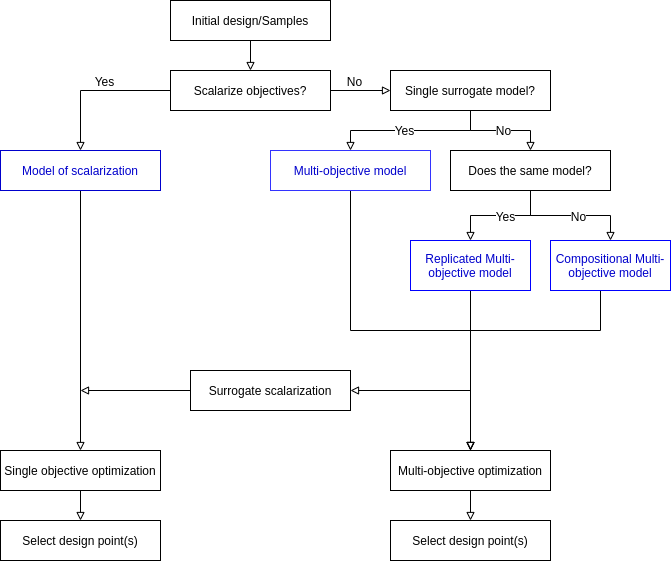
\includegraphics[width=\textwidth]{content/images/mbmo.png}
            \caption[Generalized MBMO algorithm]{Generalized MBMO algorithm}
            \label{fig:generalMBMO}
        \end{figure}


        A surrogate model is either selected randomly or due to its popularity in the area with which the problem is associated.  However, there are still some open challenges related to the ensemble of meta- models such as what should be the criterion for choosing different metamodels or how different metamodels can be used simultaneously? In addition, there are no guidelines for using different models for different objective functions \cite{SoftSurvey}.

        \cite{EngSurMod} 

        To dealing with expensive optimization problem more quickly, we can use surrogate models in the optimization process to approximate the objective functions of the problem. Approximation of solution is faster than the whole optimization process can be accelerated. Nevertheless, the extra time needed to build and update the surrogate models during the optimization process. 
        In the case of pre-selecting the promising individuals, the surrogate model is used to find the likely or drop the low-quality individuals even before they are exactly evaluated, thus reducing the number of exact evaluations.

        In the literature, the term surrogate or model-based optimization is used where, during the optimization processes, some solutions are not evaluated with the original objective function, but are approximated using a model of this function. Different approximation methods are used to build surrogate models. For single and multiobjective optimization similar methods are used. 
        These techniques typically return only one approximated value, which is why in multiobjective problems several models have to be used, so that each model approximates one objective. Some of the most commonly used methods are the Response Surface Method \cite{ResponseSurface}, Radial Basis Function \cite{Rasmussen2004}, Neural Network, Kriging \cite{Woodard00} and Gaussian Process Modeling \cite{RasmussenN10, RasmussenW06}.

        General classification \cite{MlakarPTF15}:
        Within surrogate-model-based optimization algorithms, a mechanism is needed to find a balance between the exact and approximate evaluations. In evolutionary algorithms, this mechanism is called evolution control \cite{Jin05} and can be either fixed or adaptive. In fixed evolution control the number of exact function evaluations that will be performed during the optimization is known in advance. Fixed evolution control can be further divided into generation-based control, where in some generations all solutions are approximated and in the others, they are exactly evaluated \cite{DebN07}, and individual based control, where in every generation some (usually the best) solutions are exactly evaluated and others approximated \cite{Grierson1993}. In adaptive evolution control, the number of exactly evaluated solutions is not known in advance but depends on the accuracy of the model for the given problem. Adaptive evolution control can be used in one of two ways: as a part of a memetic search or to pre-select the promising individuals which are then exactly evaluated \cite{PilatN12}.

        Surrogate used to expedite search for global optimum. Global accuracy of surrogate
        not a priority. Surrogate model is cheaper to evaluate than the objective.

        Bayesian optimization (BO) methods often rely on the assumption that the objective function is well-behaved, but in practice, the objective functions are seldom well-behaved even if noise-free observations can be collected. In \cite{bodin2019modulating} propose robust surrogate models to address the issue by focusing on the well- behaved structure informative for search while ignoring detrimental structure that is challenging to model data efficiently.

        % -------------------------------------------------------------------------------------------------
        % ------------------------------------------------        MO in Parameter tuning       -------------
        \subsubsection{Multi-objective parameter tuning}
        
            % -------------------       Surrogate-model in MOEA       
            \paragraph{Surrogate-model-based MOEA}
            In \cite{KrallMD15} proposed approaches that apply kind of surrogate assistant to evaluations and ranging new population. It allows detecting the most informative examples in population and evaluates them. 
            Identifies and evaluates just those most informative examples at the end done fewer evaluations of the real system. Another way to explore solutions is to apply some heuristic to decompose the total space into many smaller problems, and then use a simpler optimizer for each region. 

            Surrogates are also used to rank and filter out offspring according to Pareto-related indicators like the hypervolume \cite{EmmerichGN06}, or a weighted sum of the objectives \cite{TaboadaBCW07}. The problem with the methods that use hypervolume as a way of finding promising solutions is the calculation time needed to calculate the hypervolume, especially on many objectives. Another possibility is described in \cite{Li2009}, where the authors present an algorithm that calculates only non-dominated solutions or solutions that can, because of variance, become non-dominated. 
            
            GP-DEMO \cite{MlakarPTF15} The algorithm is based on the newly defined relations for comparing solutions under uncertainty. These relations minimize the possibility of wrongly performed comparisons of solutions due to inaccurate 
            surrogate model approximations. Using this confidence interval, we define new dominance relations that take into account 
            this uncertainty and propose a new concept for comparing solutions under uncertainty that requires exact evaluations 
            only in cases where more certainty is needed.


            % ------------------        Surrogate-model with MOEA       
            \paragraph{Surrogate with MOEA}
            Kind of extending the search stage of MOEA with surrogate to simulate evaluation of population. It transform the problem of searching a new better population to improving general hypothesis of how and where Pareto set presented.  

            In surrogate-model-based multiobjective optimization, approximated values are often mistakenly used in the solution comparison. As a consequence, exactly evaluated good solutions can be discarded from the population because they appear to be dominated by the inaccurate and over-optimistic approximations. This can slow the optimization process or even prevent the algorithm from finding the best solutions \cite{MlakarPTF15}. 
            
            % ------------------        Compositional architecture       
            \paragraph{Compositional architecture}
            We could describe compositional-based surrogate optimization as compound grey-box system whit a lot of open research areas where surrogate should improve, managing portfolio, compare of predictions Pareto fronts. 
            As a developer, you can be focused on a specific problem and don't know how to implement other components. This is one of the main advantages of the described approach.
    
            \paragraph{Compositional surrogates}
            Can the same single-objective models be equally applied to various types of problems in multi-/single-objective optimization?
            When there is no correlation between the objectives, a very simple way to solve this kind of problem is to build independent models, i.e. one for each objective, and then to use those models to simultaneously extrapolate possible solutions with MOEA. Nevertheless, the output values correlated, but an often naive way to build multiple models that able to extrapolate complex objective space is often given good results.  
    
            Later research generalized this approach. MOEA/D (multiobjective evolutionary algorithm based on decomposition \cite{ZhangL07}) is a generic framework that decomposes a multi-objective optimization problem into many smaller single problems, then applies a second optimizer to each smaller subproblem, simultaneously.
    
            With multiple models, their flaws can combine, as well as the time required to build the models. In memetic algorithms, especially if the surrogate model is not very accurate, a local optimum can be found instead of the global optimum. But in terms of parameter tuning, this point should be better than a predefined sampling plan. Evaluation of this prediction improve surrogate model quality in the near-optimal area and improve prediction in the next round.
            For example, OEGADO \cite{ChafekarSRX05} creates a surrogate model for each of the objectives. The best solutions in every objective get also approximated on other objectives, which helps with finding trade-off individuals. The best individuals are then exactly evaluated and used to update the models.
        

        % --------------------------------------------------------------------------------------------
        % ------------------------------------------------     Domain-specific Surrogate model      
        \subsection{Domain-specific problem}
        With gain to find the best solution with less effort surrogate models is domain-specific. It's mean that from two surrogate models in two different problems the best surrogate is changing. It could interpreter as Non-free lunch theorem in model-based optimization. If we extend this argument then the same optimization problem in different parameter tuning iteration could be interpreted as another optimization problem. This means that to reduce effort and increase the convergence of an algorithm we should change the surrogate model depend on how much samples do we have. As one would expect, no approximation method is universal.
        This leads us to use a portfolio with surrogate models. As a negative consequence, the model fitting additional introduces an additional overhead into the optimization.


        % --------------------------------------------------------------------------------------------
        % ------------------------------------------------     Build surrogate model     
        \subsection{Build the surrogate model(s). Sampling plan}



        % --------------------------------------------------------------------------------------------
        % -------------------------------------------------------        Discussion       ------------
        \paragraph{Discussion}
        Example of each type of optimization. Justification solution.
        Conclusion: Design gap in optimization/parameter tuning. 
        Need to indicate optimization workflow for expensive process/experiments. 
        The argument(s) why we need a new architecture. Reference to composition architecture.

        Surrogate based optimization has proven effective in many aspects of engineering and in applications where data is "expensive", or difficult, to evaluate.

    % --------------------------------------------------------------------------------------------
    % ------------------------------      Compositional Surrogate optimization       -------------
    % --------------------------------------------------------------------------------------------


    \section{Scope of work}
        \todo{make some nice tree-diagram}

        Describe and implement workflow for multi-objective parameter tuning of the derivative-free, black-box system. Parameter estimation is costly. The proposed solutions are also suitable for single-criteria optimization. Problem Setting.

        Goal:
        \begin{enumerate}
            \item Globally optimize an objective function(s) that is expensive to evaluate. Single/Multi-objective parameter tuning
            \item Simultaneously optimization scalable objectives
            \item Components reuse. Extensibility with other frameworks
        \end{enumerate}

        Problem:
        \begin{enumerate}
            \item A large number of the target black-box evaluations
            \item Interfaces not unify
            \item Code duplication
        \end{enumerate}

        Solution:
        \begin{enumerate}
            \item Component-Based Architecture
            \item Compositional-based surrogate optimization with MOEA
        \end{enumerate}

    \chapter{Related work}\label{sec:related}

    \begin{blockquote}
        \paragraph{Intent:} This section overview other studies in the area of surrogate-based multi-objective optimization or related approach from other types of optimization. The gaps of the others should be clearly. 
        Structure:
        \begin{description}
            \item[Comparison criteria] Surrogate type, Surrogate portfolio, Solver type, Sampling size, Many-objective optimization
            \item[Short description] 
            \item[Comparable table] 
        \end{description}
    \end{blockquote}


    % --------------------------------------------------------------------------------------------
    % ------------------------------------------------          Criteria
    % --------------------------------------------------------------------------------------------

    Many existing approaches can be categorized as multi-objective optimization. That is why introduce comparison criteria for a clear and concise demarcation of the approach presented in this thesis:
    \section{Comparison criteria for related work:}
    \begin{description}
        \item[Surrogate type] Extrapolation technique for a surrogate model. Surrogate combination
        \item[Sampling plan] Collecting sampling points for building a surrogate model
        \item[Optimization] Algorithm to find a multi-objective solution(s)
        \item[Scalability] Many-objectivity. Problems with high dimensionality in objective and parameter spaces                
    \end{description}
    Important Features: Categorical variables, prior knowledge, multi-objective, feasibility constraints.

    Hear presented related works that answer questions related to the motivation of the thesis, viz the Pareto front approximation objectives for an expensive black-box function evaluation

    Sequential model-based optimization (SMBO) [3] has become the state-of-the-art optimization strategy in recent years.
    The generic SMBO procedure starts with an initial design of evaluation
    points, and then iterates the following steps: 1. Fit a regression model to the outcomes and design points obtained so far,
    2. query the model to propose a new, promising point, often by optimizing a so-called infill criterion or acquisition function,
    3. evaluate the new point with the black-box function and add it to the design.
    Several adaptations and extensions, e.g., multi-objective optimization [4], multi- point proposal [5, 6], more flexible regression models [7] or alternative ways to calculate the infill criterion [8] have been investigated recently.



    We will briefly present an overview of available software for model-based optimization, starting with implementations based on the Efficient Global Op- timization algorithm (EGO), i.e., the SMBO algorithm proposed by Jones et al. [3] using Gaussian processes (GPs), and continue with extensions and alterna- tive approaches.

    We will argue that the proposed concept from this thesis is the preferred choice for functional optimization when the evaluation cost is large.

    % Note that this approach means that

    % --------------------------------------------------------------------------------------------
    % ------------------------------------------------          Approaches
    % --------------------------------------------------------------------------------------------

    % ------------------------------------------------          Frameworks / Platforms
    \subsection{Platforms and frameworks}
        There are a lot of different projects that can handle multi-objective solutions.

        General characteristics are that they have multiple algorithms on each type of optimization and additional features that they provide. Usually, a surrogate model is predefine and injected into some algorithm for decision making.

        \paragraph{PlatEMO} \cite{PlatEMO} PlatEMO: A MATLAB Platform for Evolutionary Multi-Objective Optimization. The platform provides a plethora of optimization algorithms for multi-/many objective problems.

        % ------------------------------------------------          Algorithms
        \subsection{Algorithms. Related Software}


        \paragraph{SigOpt} build on top of cross-validation


        % ----------------         SMAC
        \paragraph{Sequential Model-based Algorithm Configuration (SMAC)} SMAC\cite{smac-2017} adopted a random forests model and Expected Improvement (EI) to model a conditional probability. It applies a local search with several starting points and picks configurations with maximal EI. The exploration property of SMAC is improved by EI on points with large uncertainty and optimal value of objective mean. However, SMAC is limited to single-criteria optimization and use predefine sampling plan.

        % ----------------         mlrMBO
        \paragraph{mlrMBO: A Modular Framework for Model-Based Optimization of Expensive Black-Box Functions} Bischl et al.,\cite{mlrMBO} provide a framework with a focus on multi-criteria parameters optimization. MlrBO extends the MBMO procedure for mixed and hierarchical parameter spaces. For the surrogate, that project allows any regression learner from $mlr$ library. That is why a bagging method can be applied to regression models to retrieve model error in $mlr$. This framework enables proposing several points for evaluation. However, it doesn't provide a combination of different surrogates into one model. Example of provided algorithm: ParEGO
            % ----------------         ParEGO
            \paragraph{ParEGO} scalarization based multi-objective algorithm \cite{Knowles06}. Classical single-objective algorithm of Jones et al. EGO was extended to a multi-point proposal by repeat algorithm several times with randomly change scalarizations weights in each iteration. The idea of algorithm based on Kriging/Gaussian process regression model and multiple single objective optimization processes on scalarized objectives guaranteeing that multiple points on the Pareto-optimal front are found.


        % ----------------         Distributed Surrogates
        \paragraph{An Evolutionary Algorithm with Spatially Distributed Surrogates for Multiobjective Optimization} Amitay et al.,\cite{DistrSurr}presented in their paper an evolutionary algorithm with spatially distributed surrogates (EASDS). Surrogates periodicaly validated and updated. Radial Basis Function Networks were used as the surrogate model for each partition from samplings points. Spatially Distributed Surrogate models are created for all the objectives and than evaluated by NSGA-II. The authors describe that their approach achieves better results than single global surrogate models showing an advantage from using multiple surrogates. However, authors evaluated there algorithm only on bi-objective problems
 
        % ----------------         Hybrid surrogate
        \paragraph{A hybrid surrogate-based approach for evolutionary multi-objective optimization} Rosales-Pérez et al.,\cite{HybridSurrRCG} proposed an approach based on an ensemble of Support Vector Machines. Authors describe a model selection process or hyperparameters selection of SVM based on cross-validation technique and fother injection to the surrogate ensemble. 
        Incremental development of the ensemble, that includes new information obtained during the optimization and stores previous models. The training of a new model carries the grid search of SVM Kernel types to find one with the least expected generalization error. This paper presents a model selection process for determining the hyperparameters for each SVM in the ensemble.

        % ----------------         Surrogate Search
        \paragraph{Efficient Multi-Objective Optimization through Population-based Parallel Surrogate Search} Akhtar et al.,\cite{akhtar2019efficient} introduce a multi-objective optimization algorithm for expensive functions that connect iteratively updated several surrogates of the objective functions. Feature of this algorithm is high optimization for parallel computation. An algorithm combines Radial Basis Function (RBF) approximation, Tabu and local search around multiple points. Authors present an algorithm that can theoretically be applicable for hight dimensional space and many-objective problems.

        % ----------------         GALE
        \paragraph{GALE: Geometric Active Learning for Search-Based Software Engineering} Krall et al.,\cite{KrallMD15} developed algorithm that uses PCA and active learning techniques to step-by-step approximation and evaluating the most informative solutions. The main features of GALE are active learning in geometrically analysis perspective regions in search space to select most prospective candidates.

        % ----------------         Hypermapper
        \paragraph{Hypermapper} Luigi Nardi et al. \cite{nardi2019practical} presented multi-objective black-box optimization tool. Some features of their approach are prior knowledge, categorical variables, feasibility and good adaptation to embedded devices. They train separate models, one for each objective and constarints. Then merge it with random scalarizations (Tchebyshev/ Linear scalarization). Next, the Bayesian model leads local search algorithm to explore Pareto optimal points.  

        % ----------------         Hierarchical surrogates
        \paragraph{Evolutionary optimization with hierarchical surrogates} Xiaofen Lu et al. \cite{LuST19} apply different surrogate modelling techniques based on motivation on optimization expensive black-box function without any prior knowledge on a problem. They used a pre-specified set of models to construct hierarchical surrogate during optimization. Also, for verification of surrogate used general accuracy of the high-level model. The whole process of the proposed method split to accumulate training samples and model-based optimization, that means that the sample plan is static and require prior information about the problem.

        %! A mathematic analysis was given in this paper to show that the hierarchical surrogate structure can be beneficial when the accuracy of the high-level model is larger than 0.5.
        % !However, one modeling technique might perform differently on different problem landscapes.


        \begin{table}
            \centering
            \caption{Related work}
            \begin{tabular}{|l|l|l|l|l|l|}
            \hline
            
             & Surrogate & Optimization Algorithm & Sampling plan & Scaling of test problems & Year \\ \hline
            Distributed Surrogates (EASDS) & Radial Basis Function Networks, clustering & NSGA-II & Static: Random samples & 2 obj & 2007 \\ \hline
            Hybrid surrogate-based approach & Ensemble of Support Vector Machines & NSGA-II & Static: Latin-hypercube samples & 2 obj & 2013 \\ \hline
            mlrMBO & Regression model(s) & Single-/Multi-opt algorithm & Static & ? & 2017 \\ \hline
            SMAC & Eandom forests + Expected Improvement & Local search & Static & 1 obj & 2017 \\ \hline
            Parallel Surrogate Search (MOPLS-N) & Radial Basis Function & Tabu and local search & Static & 2 obj & 2019 \\ \hline
            GALE & PCA-approximation + linear models & MOEA/D & Static & 2-8 obj & 2015 \\ \hline
            Hypermapper & Randomized decision forests & Scalarizations + Gaussian Processes + Local search & Static & 2 obj & 2019 \\ \hline
            ParEGO & Kriging/Gaussian process regression & scalarizations + EGO & Static: Latin hypercube samples &  & 2006 \\ \hline
            Hierarchical surrogates & Dinamic hierarchical surrogate & EA & Static & 1 obj & 2019 \\ \hline
            
            \end{tabular}
        \end{table}

    % --------------------------------------------------------------------------------------------
    % ------------------------------------------------          Approaches
    % --------------------------------------------------------------------------------------------
    \subsection{Conclusions}


        \begin{enumerate}
            \item One modeling technique might perform differently on different problem landscapes. \cite{LuST19}
            \item Surrogate model can be useful when the accuracy is larger than 0.5. \cite{LuST19}
        \end{enumerate}





        % However, it lacks fundamental features that makes it ineffective in the presence of applications with non-feasible designs and prior knowledge.


        % Our work is similar in nature to the approaches adopted in the Bayesian optimization literature [27]. Example of widely used mono-objective Bayesian DFO software are SMAC [15], SpearMint [30], [31] and the work on tree-structured Parzen estimator (TPE) [6]. In particular, the use of a full Bayesian ap- proach will help to leverage the prior knowledge by computing a posterior distribution. Exploration of additional methods to warm-up the search from the design of experiments literature

        % \paragraph{Hyperopt}




        % Based on a survey\cite{SoftSurvey} there still exist such as:
        % \begin{itemize}
        %     \item 
        % \end{itemize}


        % Some features of their approach are 


        % We extend the idea of stochastic RBF to be suitable for the algorithm con- figuration task. It is a model-based algorithm that cycles from emphasis on the objective to emphasis on the distance using a weighting strategy. 
        
        % The main advantage of LHS is that it does not require an increased initial population size for more dimensions.


        % exploration, exploitation and diversification during each algorithm iteration.



        % To our knowledge, there exists no research that investigates how deep networks affect the performance of surrogate-assisted multi-objective evolutionary algorithms. If neural networks were used, the approaches usually adopted only one hidden layer. Additionally, we can also see that there exists a multitude of ways a surrogate model can be integrated into an evolutionary algorithm

        % Previous studies have shown that the choice of modeling technique can highly affect the performance of the surrogate model-assisted evolutionary search.

        % However, one modeling technique might perform differently on different problem landscapes. Without


        % OpenTuner is different from our work in a number of ways. First, our work supports multi-objective optimization. Second, our white-box model-based approach enables the user to understand the results while learning from them. Third, our approach is able to consider unknown feasibility constraints. Lastly, our framework has the ability to inject prior knowledge into the search. The first point in particular does not allow a direct performance comparison of the two tools.

        % over the entire space would result in a waste of samples.


        % This is especially the case for a SMBO

        % The black-box function can be more complex, for example a machine learning pipeline which includes preprocessing, feature selection and model selection.


        % Consequently, the advantage of the multi-objective candidate generation to produce a set instead of single points is not only used for improving the exploration of the decision space, but also for obtaining a well-spread batch of solutions.

    \chapter{Concept}\label{sec:concept}

    % \begin{blockquote}
    %     \paragraph{Intent:} General reminder and answer of RQ's
        
    %     Structure:
    %     \begin{description}
    %         \item[1. Surrogates models combinations] Surrogate model is not universal. Domain-specific $\rightarrow$ Surrogate model portfolio 
    %             \begin{enumerate}
    %                 \item Surrogate model is not universal. Domain-specific $\rightarrow$ \textbf{Surrogate model portfolio}
    %                 \item Objectives have different complexity surface $\rightarrow$ Surrogate model is not universal $\rightarrow$ Describe objectives independently. \textbf{Heterogeneous/Composition surrogate model} 
    %             \end{enumerate}
                  
    %         \item[2. Dynamic sampling plan] Use sampling plan while surrogate is not valid
    %             \begin{enumerate}
    %                 \item Surrogate Validation. Stages and thresholds
    %                 \item Metrics
    %             \end{enumerate}

    %         \item[3. Scalability] Compositional surrogates in many-objective space
    %             \begin{enumerate}
    %                 \item Problem: Random solver on high dimensional space $\rightarrow$ Solution: Light surrogates 
    %                 \item Solving problem in subset of dimensions
    %                 \item Categorical parameters*
    %             \end{enumerate}

    %         \item[4. Discussion] General Conclusions. Infill criteria for Pareto-optimal solutions
    %     \end{description}
    % \end{blockquote}

    \epigraph{``All models are wrong but some are useful``}{\textit{– George Box}}

    This section presented a general idea of a improvement in the surrogate-based optimization for black-box function. 

    The usual optimization problem is a trade-off in producing the best possible multi-objective solution with less effort. Because we consider expensive function, an optimization effort, first of all, means evaluation budget. Each of these evaluations can require much time, energy, or other resources. That is why the main multi-objective comparison criteria are convergence to the Pareto frontier with a limited evaluation budget. It also takes into account the ratio of non-dominant solutions to the total number of measured configurations and their distribution on the Pareto frontier. In this thesis, under solving a multi-objective problem, we intend to find a set of none-dominated points that cover a wide range of objectives values and close as possible to the real Pareto front. If evaluations of the problem are expensive, the real count of experiments could be reduced throw applying a multi-objective algorithm on a surrogate model. This technique is the preferred choice for functional optimization when the evaluation cost is high.

    While multiple algorithms could be applied, we selected \gls{moea} as default optimization techniques for the surrogate models. The advantage of \gls{ea} is that it could be easily modified and it could operate on a set of solutions candidates, that are well-fitted to approximate the Pareto-front. Finally, evolutionary algorithms can estimate highly complex problems in various use-cases.


    %? The main objective of this part is to provide a thorough treatment of multi-objective parameter tuning with evolutionary algorithm(s)


    % The solution techniques and parametric selections however are usually problem-specific. \cite{abs181207958}
    % --------------------------------------------------------------------------------------------
    % ------------------------------------------------     RG1: Models combinations     
    % --------------------------------------------------------------------------------------------

    \section{Surrogates models combinations [RQ1]}

        Let us address the main issue we have observed in multi-objective optimization. Base on the statement that the surrogate model is domain-specific, the central idea of the thesis is introduced as the model variability \emph{in} a surrogate model and the extensibility \emph{with} surrogate hypotheses.

        % ------------------------------------------------     Compositional model       
        \subsection{Compositional Surrogate Model}
            The concept of the compositional surrogate means a combination of the multiple simple models that simulate the several objectives independently at the same time. Dividing optimization problems to several parts improves the variability of surrogates and accordingly, the possibilities to improve the solution.
            Besides, a significant advantage of the compositional surrogate is a possibility to extend the single-objective parameter tuning to the multi-objective task. This provides the opportunity to reuse single-criteria models for multi-criteria optimization and dynamically reconstruct problem representation from mixed parts.
            
            % Nonetheless, the surrogate model is not universal to describe objectives independently. 

            That approach should be capable, outperform static models in adaptation to a real black-box problem with the unknown objective surface. For example, a user could represent his domain knowledge as preferring to a concrete combination of the surrogate models or calibrate it during optimization. 
            
            In this thesis, the \emph{compositional model} means a surrogate model that combines various surrogates models for each optimization objective. The \emph{surrogate hypothesis} refinement is also used to emphasize on the fact that the surrogate model can completely describe all criteria from the objective space.

            % ------------------------------------------------     Scalability     
            \subsubsection{Scalability}
                In practice show that an MOEA is challenging to scale. For many-dimensional problem, more than 10 objectives random solver gain better solution than MOEA. Furthermore, surrogate models also suffer from this. For instance, complexity ob Krigin/Bayesian model increase exponential with growing samples size and dimensionality.
                % ! \todor{examples how to solve it, related work}

                The compositional model could improve the solution by a precisely select group of surrogates to describe problem landscape. Each surrogate model could extrapolate one or subset objectives and together with other model provide a complex hypothesis of how a parameter and objective spaces related.

                As a result, it should allow us to build a useful surrogate model to make a quality many-objective decision in parameter tuning. 

            % -------------------------     Categorical parameters      
            \subsubsection{Categorical parameters} Multi-objectivity and a real/ordinal/categorical parameters are essential for real parameter tuning. There are known two basic approaches to implement this functionality: decision tree or feature encoding and fit arbitrary model. Most related works used native models that support categorical features because it is interpretative and can transform prediction backwards. 
            On the other hand, feature encoding is used to support a categorical parameter for generic models. Coding features for a surrogate model can transform those in a meaningful form, understandable for a surrogate model. Encoding represents a feature in an alternative form that helps model instantiation relation and a correlation between features. Based on this inner interpretation model can predict the values of labels based on a parameter vector. The problem occurs in reverse interpretation of these optimal predictions in the context of parameter space. Often a found solution is not a feasible point from parameters space. As a possible solution, it partly transforms problems in multiple classification tasks and then considers there relation as optimization with continuous probability [TPE]. 
            For the general surrogate model with mixed parameters, we can solve a problem orthogonally with multiple optimizers.  Then general idea consists in sequentially applying several algorithms that use previous results. For example, encode features and fit models as usual. First, apply local search that can evaluate only valid parameters. The solutions found may be satisfactory but not optimal.  The next step is a genetic algorithm that uses the result of the previous algorithm, namely the optimal categories values. The multi-algorithm help achieve the most significant values in the remaining parameters. 

            Such a concept is vital for expensive multi-criterion optimization when the solution space is mixed and has an overwhelming number of real values. 
            
        
        % ------------------------------------------------     Portfolio      
        \subsection{Surrogate model portfolio}
            With gain to find the best solution with less effort surrogate models is domain-specific. It's mean that there is no universal approximation model. It could be interpreter as Non-free lunch theorem in model-based optimization. If we extend this argument, then the same optimization problem with another sample set could be interpreted as another optimization problem. The search space landscape, modality and geometry may hugely differ. The complexity to restore the original problem change during optimization. It depends on how much samples are and which diversity they have.
            This means that to reduce effort and increase the convergence of an algorithm, we should change the surrogate model depend on how much samples do we have. As one would expect, no approximation method is universal. Hence, this leads us to use a portfolio with surrogate models. As a negative consequence, the model fitting introduces an additional overhead into the optimization. 
        
            With the flexibility that provides a compositional system to combine several models, that is valuable to produce several variants of compositions from available surrogates. This functionality requires validation criteria to discard those that are not valid and comparison metrics to range and combine the best ones. There are created many hooks to combine and solve surrogates models. These placeholders give flexibility to the combination of hypotheses, testing, and solving/optimization. Bagging or ensemble technique can be applied to both steps: the surrogate models and the optimization algorithms.

            Besides, it grates motivation to use the latest state-of-the-art algorithms and models together because the modular structure of the compositional model and portfolio allows using it as hooks for optimization.  

    % --------------------------------------------------------------------------------------------
    % ------------------------------------------------     RG2: Sampling plan     
    \section{Sampling plan [RQ2]}
        For expensive optimization problems, it would be useful to modulate a problem using quite a small number of most informative examples. Nonetheless, almost sequential model-based approaches use a static sampling plan. Under the sampling plan may also be assumed randomized designs in design-of-experiment(DOE). If the oracle does not determine the required optimal samples, it can lead to unnecessary waste of valuable evaluation attempts. 
        
        The general idea of how to solve this problem lay on relating initial sampling design to validation the surrogate models. An optimization search is guided by sampling design until that moment when valid surrogate model is presented (Figure \ref{fig:concept_sampling}). Validity means that surrogate approximation could be useful for efficient global optimization.

            % ==== Sampling plan
            \begin{figure}
                \centering
                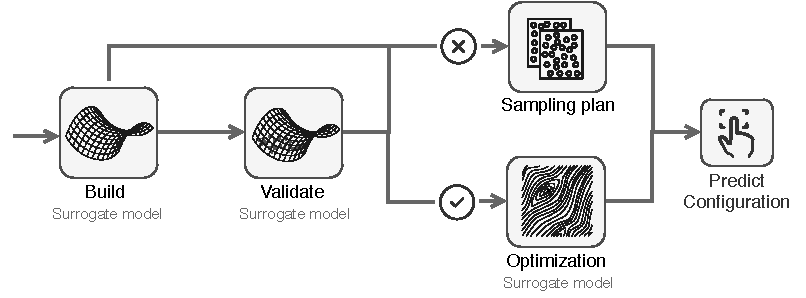
\includegraphics[width=\textwidth]{content/images/dinamic_sampling_plan}
                \caption[Non-dominated points]{Concept of a sampling plan dependency and model validation. A sampling plan is used if there is no valid model that can be useful for optimization purpose.} 
                \label{fig:concept_sampling} 
            \end{figure}      

        % -------------------------     Surrogate Validation      
        \subsection{Surrogate Validation}
        It is necessary to sacrifice a small portion of samples to check the quality of the surrogate model. Based on validation results, we can discard inadequate models and elaborate evaluate the solutions from valid models. If neither model is valid, this means that the best solution right now is a prediction from the sampling plan. This decision is repeated until a valid surrogate model is obtained.
        In the context of sequential model-based optimization, a common misconception lay in prefer global accuracy score over the score in the optimal region. That is why evaluation surrogate validity based only on the coefficient of determination(R2) metrics is incorrect \cite{nardi2019practical}. Global accuracy metric can be used as a threshold value for exceeding which the model becomes not valid even with additional estimations.  

            % ==== train\valid\test
            \begin{figure}
                \centering
                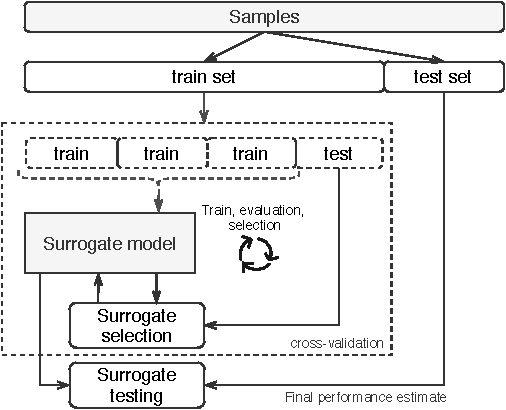
\includegraphics[width=10cm]{content/images/cv}
                \caption[Cross-validation: exploration vs exploitation]{Validation surrogates models. Cross-validation loop performs selection models based on global accuracy; Successful models perform on a test set with a focus on optimization region.} 
                \label{fig:cv}   
            \end{figure}

        The central concept for surrogate validation lay in adaptation best practices from the machine-learning community for evaluation estimator's performance. 

        Validation should show how well the model extrapolates the available experiments and how well it can evaluate the data that is not seen. In the case of validation a several models, results could have not a representative performance if data split only to train/test set.  There is a risk of overfitting on the test data. It means that the test set 'leak' to train set and final metrics does not report on the surrogate achievement. 
        Deal with this problem, yet another portion of samples can handle as a so-called 'validation set.' This new set is used for model selection independently from the test set. When models are selected, final evaluation can be done on the test set. However, partitioning the available samples into three sets, are drastically reduce the number of points which can be used for learning the model. Moreover, results can depend on a selective random decision for the samples splitting.
        
        The solution is might be cross-validation(CV, Figure \ref{fig:cv}). This is a procedure that avoids a separate validation set and divides test samples to \textit{k} equal folds. Set of folds are used to train model and in \textit{k} rounds, a new fold selected as a test set. The performance measure by cross-validation is the average of the values computed in the loop. This approach can be computationally expensive, but requires fewer samples. 
        
        As s result, the concept of a surrogate validation based on two sequential stages:
        \begin{enumerate}
            \item \textbf{Cross-validation.} Evaluate that model performs well to generalize landscape. Select candidates that have enough accuracy.
            \item \textbf{Surrogate testing.} Final evaluation performs on the test set that shows accuracy on the region of interests. In the context of multi-objective optimization, it is non-dominated samples.
        \end{enumerate}
        
        The decision on which surrogate model is better made based on the information from all stages. If the model does not have a sufficient threshold, it is rejected as not valid. If there is no valid model, the assumption of the next configuration is accepted from the sapling plan (Figure \ref{fig:concept_sampling}).

        % overfit - underfit
    
        % metrics comparison


    % --------------------------------------------------------------------------------------------


    % --------------------------------------------------------------------------------------------
    % -----------------------------------------------------       Discussion      ----------------
    \section{Discussion}

        In this thesis, proposed approach for combination surrogates for multi-objective optimization and dynamic sampling plan based on surrogate validation.

        As a reply to RG1 we provide two answers: 1.) Combination complex surrogate model from surrogates on objectives 2.) Comparison of multiple surrogates in the portfolio to select the best one or generate an ensemble of results from all applicable variants.

        % -----------------------------------------------------      Infill criteria       
        \paragraph{}{Infill criteria}
        In the case of MOEA, solution of algorithm present as non-dominated final population. Based on unbiased, multi-objective criteria, they all uniformly could be presented as a prediction to the next evaluation. They represents current solution based on the surrogate model. Nevertheless, there is prior knowledge available in samples which can be taken into account. To reduce the number of candidates in the population, it is possible to deny those in which the distance to the nearest available sample is less than their average distance.
        So there are two strategies for predicting from a population:
        \begin{itemize}
            \item Prior and posterior knowledge. Based on changing metrics in available and proposed solutions
            \item Posterior knowledge. Proposed solutions are all equal
        \end{itemize}


        
        % -----------------------------------------------------       Conclusions       
        Also, to the best of our knowledge, has not been previously or stingy reported in the efficient multi-objective optimization.
        Contribution:
        \begin{itemize}
            \item Surrogate combination/composition with heterogeneous models
                \begin{itemize}
                    \item Surrogate models portfolio
                    \item Compositional surrogate model
                    \item Combination of different(orthogonal) solvers
                \end{itemize}
            \item Surrogate portfolio. Search a better hypothesis  for a specific problem at a particular stage of parameter tuning
            \item Metric combination for evaluation Pareto optimal points
            \item Samples size depends on model(s) validity
            \item Concepts
                \begin{itemize}
                    \item Combination of different(orthogonal) solvers
                    \item Infill criteria for prediction selection
                \end{itemize}
        \end{itemize}

        We argue that the proposed concept from this thesis is the preferred choice for functional optimization when the evaluation cost is large.


        Our work is similar in constitution to the approaches adopted from the expensive MBMO \cite{SoftSurvey} with a modular framework structure that includes a surrogate portfolio. We extend the idea of model selection and k-fold cross-validation to verify how a surrogate(s) model might operate differently on various problem sceneries. To our knowledge, there exists no research that investigates how to make a composition of several surrogate models and use it in a portfolio. Also, there is an open question how this method scales.


        % structures include more than one possibility, as described above. Nevertheless, this level

        % Finally, another aspect worth mentioning is the fact that GSM appears in more than one cell. Indeed, hybrid methods


        % where the algorithms are allowed to query an oracle for additional data to infer better statistical models


        % They also reported that a speedup of a factor of 10 can nevertheless be obtained.



        % With multiple models, their flaws can combine, as well as the time required to build the models. In memetic algorithms, especially if the surrogate model is not very accurate, a local optimum can be found instead of the global optimum. But in terms of parameter tuning, this point should be better than a predefined sampling plan. Evaluation of this prediction improve surrogate model quality in the near-optimal area and improve prediction in the next round.
        % We could describe compositional-based surrogate optimization as compound grey-box system whit a lot of open research areas where surrogate should improve, managing portfolio, compare of predictions Pareto fronts. 
        % As a developer, you can be focused on a specific problem and don't know how to implement other components. This is one of the main advantages of the described approach.

        % less prone to overfitting
        % To our best knowledge, we are the first to make this simple observation, which can be applied to improve any Bayesian hyperparameter
        % optimization method.
    \chapter{Implementation}

\begin{blockquote}
    \paragraph{Intent:} Details of implementation. Requirements: reusable components, unify interfaces. Duck typing 
    
    Structure:
    \begin{description}

        \item[1. Compositional surrogate model] heterogeneous model combination on each objective
        \begin{enumerate}
            \item Model-union class. Stacking surrogate. Tree composition
        \end{enumerate}

        \item[2. Surrogates validation] When the surrogate model can be helpful?
        \begin{enumerate}
            \item Validation workflow. Adaptation from Data science
            \item Hypothesis portfolio validation and combination
            \item Stages and thresholds
        \end{enumerate}

        \item[3. Solvers] Optimization algorithms. Solve problem based on surrogate model(s)
    \end{description}
\end{blockquote}
% ================================================================================================

This section describes the details and decisions in the implementation of the proposed thesis concept. Implementation should be flexible and usable. Consist of buildings blocks with consistent interfaces. Achieve a wide diversity of solving problems within extension from other algorithms and frameworks. Based on best practice \cite{buitinck2013api}, the implementation accepts the following principles:
\begin{itemize}
    \item \textbf{Components.} Simple and efficient, reusable in various domains. Whenever possible, new functionality is implemented and composed from existing building blocks.
    \item \textbf{Separation of concerns.} Implementations of surrogate models and optimization algorithms are unrelated and interchangeable. 
    \item \textbf{Non-proliferation of classes.} Samples and Datasets are represented as arrays or data frames. Hyper-parameter names and values are represented as standard Python strings or numbers whenever possible. This keeps components easy to use and easy to combine with other libraries \cite{buitinck2013api}.
\end{itemize}


The next dependencies are chosen to achieve the above mention principles:
\begin{description}
    \item \textbf{Scikit-learn} \cite{art-scikit-learn} is one of the most popular machine learning framework that accomplishes with a variety of learning tasks. The critical features are excellent documentation and reusable components in various contexts. Extensibility and consistent interfaces lead that the library has gathered a large community. Scikit-learn integrates well with many other Python libraries. 
    \item \textbf{pygmo2} \cite{francesco_biscani_2019} is efficient parallelization scientific library for local and global optimization. Key features of their project are efficient implementations of bio-inspired and evolutionary algorithms and unified interface to optimization algorithms and problems. 
\end{description}

               



% \paragraph{Reusability in parameter tuning} Parameter tuning can be splitted down into steps that are common for the many/single-objective optimizations. Each step in optimization workflow has variability via implemented interfaces. Single-objective hypotheses can be combined for multi-objective optimization with compositional design. API of metric-learn is compatible with scikit-learn, the leading library for machine learning in Python. This allows to use all the scikit-learn routines (for pipelining, model selection, etc) with metric learning algorithms through a unified interface.


% \paragraph{Inner interfaces} Supervised learning consists in learning the link between two datasets: the observed data X and an external variable y that we are trying to predict, usually called target or labels. Most often, y is a 1D array of length $n samples$. All supervised estimators in scikit-learn implement a fit(X, y) method to fit the model and a predict(X) method that, given unlabeled observations X, returns the predicted labels y. Using arbitrary regression models from scikit-learn as surrogates. Problem that each optimization framework/library use inner interfaces. It is necessary to define a standard that implements best practices for extension libraries \cite{buitinck2013api}. We introduce new Model-based line for parameter tuning. 



% --------------------------------------------------------------------------------------------
% ---------------------------------------------------       Compositional surrogate      
% --------------------------------------------------------------------------------------------
\section{Compositional surrogate}
    Model-union class (Figure \ref{fig:munion}) is a place where several heterogeneous models could be combined. This class is as meta-model that wraps and aggregate estimations from several sub-models. Model-union could be combined in a tree structure with arbitrary models that support require interface. There are two estimation modes:
    \begin{itemize}
        \item \textbf{Stacking.} It is an ensemble learning technique to combine multiple regression models by a meta-regressor. The individual regression models are trained based on the whole training samples. The final label prediction is averaged from all models outputs.
        \item \textbf{Split y.} A straightforward technique to combine several regression models to multi-label prediction. The individual regression models are also trained based on the whole training samples, but final prediction produces from a model's outputs concatenation. For each model features space is common, but labels are orthogonal. This functionality allows as to produce multicriteria compositional models from combinations of single objective models.

    \end{itemize}

    % ==== Sampling plan
    \begin{figure}
        \centering
        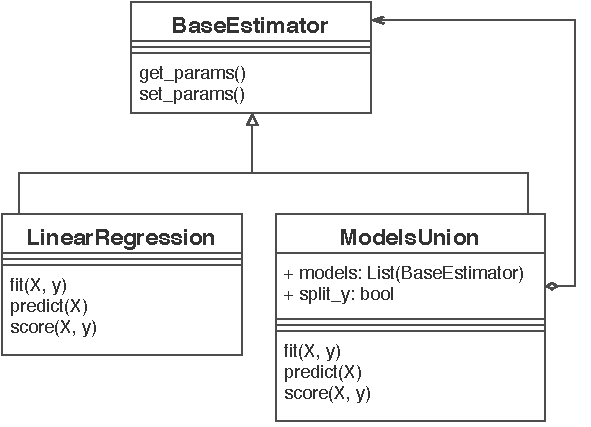
\includegraphics[width=10cm]{content/images/munion_class}
        \caption[Models-union class]{Class diagram of \textit{ModelsUnion}. Scikit-learn tends to use "duck typing", so building a model which supports require methods suffices for compatibility. Internal classes such as \textit{BaseEstimator} provide boilerplate code and is used for clarity and convenience intent.} 
        \label{fig:munion} 
    \end{figure}  

    ModelsUnion class puts the compositional model on one line with other surrogate models. It allows us uniformly validate many surrogate models and combine them in a surrogate portfolio.

% --------------------------------------------------------------------------------------------
% ---------------------------------------------------       Optimization orchestrator     
% --------------------------------------------------------------------------------------------
\section{Optimization orchestrator}
    The \textit{TutorModel} class is the orchestrator of all optimization's processes. It holds a surrogate portfolio, makes validation decisions, combines valid surrogate hypothesis and brings them together with optimization solvers (Figure \ref{fig:tutor_activity}).

    %! [ === Model product line === ]


    % ---------------------------------------------------        Validation
    \subsection{Surrogates validation}
        Each surrogate pass validation in several stages (Figure \ref{fig:simsim_activity_validation}): 1) Surrogate selection based on cross-validation results. In this stage define lower bound for overall accuracy. We notice that pass this threshold does not guarantee that surrogate is useful, but we sure that lower values detect models as useless. By default threshold \#1 defines as R2 less than 0.65. 2) Check accuracy in the region of interest. Finalist models chacks on unseen data to validate extrapolation quality and accuracy in optimal points. By default, R2 at this stage is also should be more than 0.65. Accuracy in optimal points is used for sorting champion models and corresponding solutions. Threshold's values selected from practical and theoretical use.

            % ==== activity_validation
            \begin{figure}
                \centering
                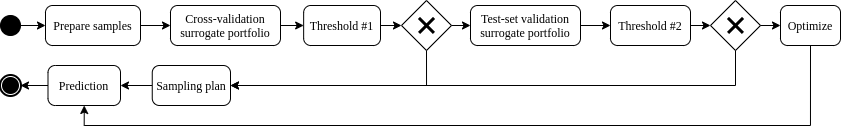
\includegraphics[width=\textwidth]{content/images/simsim_activity_workflow}
                \caption[General workflow activity]{General optimization workflow for model-based optimization iteration with validation in two stages.}
                \label{fig:simsim_activity_validation}
            \end{figure}

        The test set by default is 25\%. On left 75\% used cross-validation in 4 rounds. It means that gained four folds of samples and models training perform in three folds and testing on the fourth fold. It performs results for select or rejects surrogates combinations. After on test set gain information about the quality of possible solutions from surrogate 


    % ---------------------------------------------------        Portfolio        
    \subsection{Hypothesis portfolio}
    In general, surrogate models can be divided into two groups: a multi-output model for all objectives and compositional model with single-output models. All models pass validation equally, but after cross-validation single-objective models should combine in the complex surrogate hypothesis. 
    Ultimately, all objectives should be restored from valid surrogates and if some objective dimension has more models than other, last duplicate themselves to fill a gap. After complete restoring, compositional models with multi-output models validate further on the test set.

    % In the case of mixed surrogates models portfolio, validation pass in two groups: multi-objectives and single objective surrogates. In single-objective surrogates group must additionally restore complite hypotheisis for the multi-dimensional objective surface.

        % ==== Figure
        \begin{figure}
            \centering
            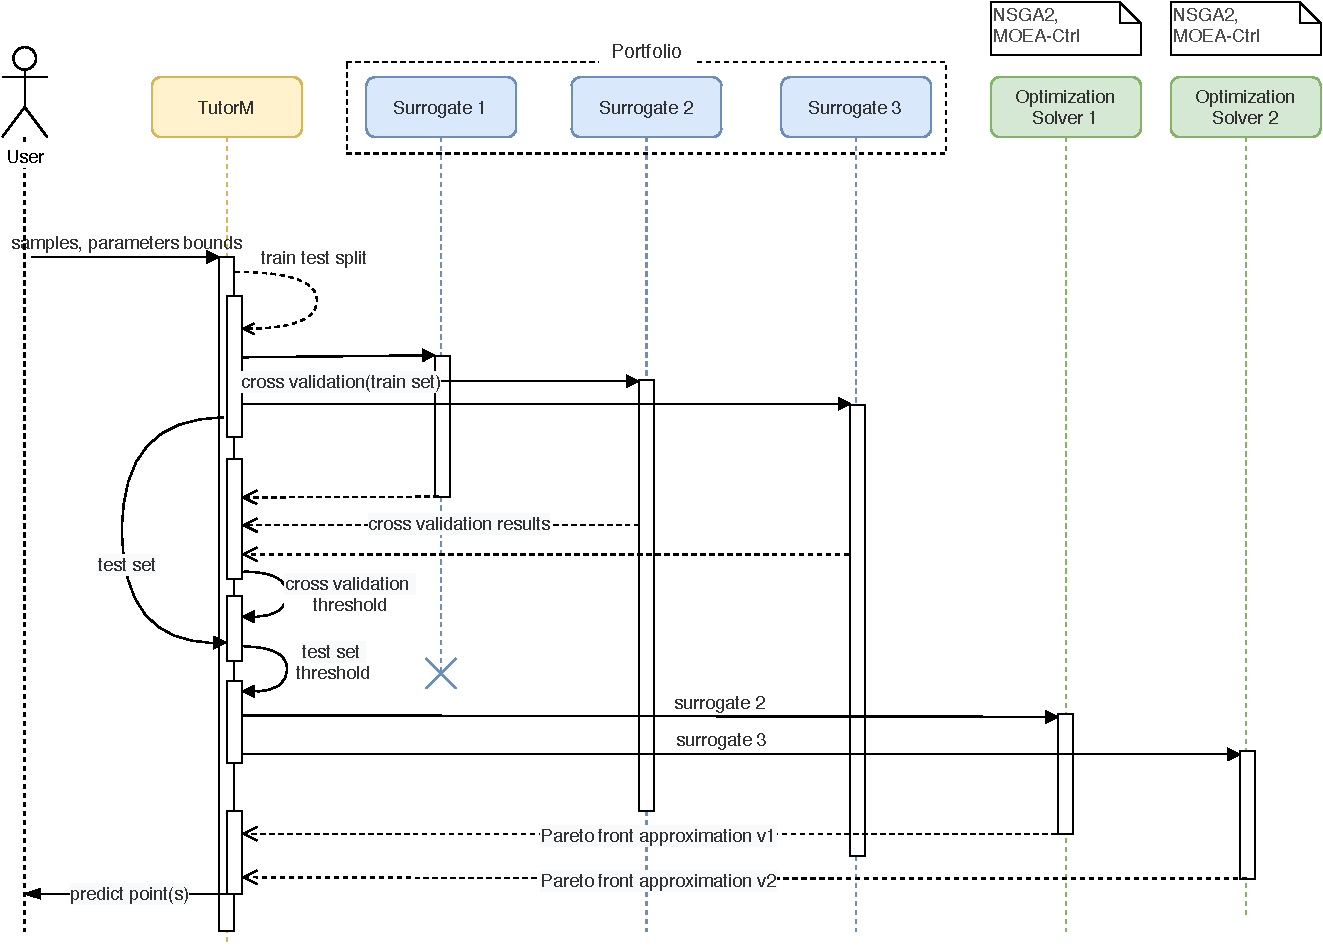
\includegraphics[width=\textwidth]{content/images/portfolio_validation_solv}
            \caption[Portfolio validation activity]{This is a validation and optimization workflow of several surrogates}
            \label{fig:tutor_activity}
        \end{figure}



    % ---------------------------------------------------        Sampling strategy
    \subsection{Sampling strategy} In many practical problems, only a restricted budget is spendable. Each evaluated point should be informative to reduce cost and improve interpolation by models. The most straightforward method of sampling design is a random witch for small sample sizes, that often produce clusters of samples. Conversely, there are also quasi-random distributions that produce informative samples that cover space more evenly. Most popular algoruthms are Sobol\cite{Sobol1999} and Latin hypercube sampling. 
    Out of the box, we provide Sobol sampling and random sampling.
    
    
    % Oversampling and undersampling in data analysis. Alleviate imbalance in the dataset. 
    % Imbalance in dataset is not always a problem, more so for optimization tasks. 

    % The main gain for models not to provide best accuracy on all search space but provide possible optimum regions.
    % Accuracy in prediction optimal regions or points from there will direct the search in the right direction.

    % Predictor variables can legitimately over- or under-sample. 
    % In this case, provided a carefully check that the model assumptions seem valid.

    % for other set of parameters, and make a choice from more diverse pool of models.

% --------------------------------------------------------------------------------------------
% ---------------------------------------------------       Solvers      
% --------------------------------------------------------------------------------------------
\section{Optimization solvers}


    Solvers role is to apply an optimization algorithm on the surrogate and find a solution(s). Most solvers implemented with Multi-objective evolutionary algorithms such as NSGA2, MOEA/D, Multi-objective Ant Colony Optimizer (MACO) or Nondominated Sorting Particle Swarm Optimizer (NSPSO). 
    Specifically added solver with a combination of several multi-objective genetic algorithms with a shared population (MOEA-Ctrl).

    Accordingly, on this step, a version of the solver with a scalarization of surrogates values possible witch optimize with any optimal heuristics. In this case, only one optimal point is obtained from the Pareto front, so the process must be repeated as many times as necessary to obtain the required count. 

    Optimization framework requires the definition of custom problems. Optimization algorithm receives the surrogate model as a parameter and builds custom optimization problem on it. In the case of a genetic algorithm, gain the perspective population of parameters, that could be selected as a Pareto front approximation. If several surrogates valid - several Pareto-front approximations obtain. There are two approaches to select the most informative solutions: 1) select Pareto approximation from surrogate with the highest accuracy in non-dominated points. 2) Assume that all approximations are valid and all points could be selected. In this case, intersection predictions from samples have a higher probability of being selected

    For singl-objective problem was adopted Extended Ant Colony Optimization algorithm (gaco). Feature of this algorithm consist in applying Gausian process regresion to generate future generations of ants. 

    All default solver allgorithms are implemanted in pygmo2 \cite{francesco_biscani_2019}.
    % Optimization algorithms. MOEA. A Python platform\cite{francesco_biscani_2019}  to perform parallel computations of optimisation tasks (global and local) via the asynchronous generalized island model.

    % decorators for single-objective solver with multi-objective surrogate 








% ----------    Designing a Sampling Plan
% \paragraph{Designing a Sampling Plan} The most straightforward way of sampling a design space in a uniform fashion is by \cite{EngSurMod} means of a rectangular grid of points. 
% Random sampling has the downside that for small sample sizes, there is often signficant clustering of samples, which is not ideal for interpolation since clustered samples can be wasteful. Instead, often a better option is to use a Latin hypercube, which enforces a condition that sample bins may not share the same coordinates for any coordinate axis







% Without automated tools, it can take days for experts to review just a few dozen examples.  In that same time, an automatic tool can explore thousands to millions to billions more solutions. People find it an overwhelming task just to certify the correctness of conclusions generated from so many results.


% Managing complex execution Strategies


% The simplifications are mean to discard the superfluous details that are unlikely to generalize to new instances. However, to decide what data to discard and what data to keep, you must make a hypothesis. For example, a linear model makes the hypothesis that the data is fundamentally linear and that the distance between the instances and the straight line is just noise, which can safely be ignored.



% sklearn 'duck typing'. This means that estimators are defined by interface, not by inheritance, where the interface is entirely implicit as far as the programming language is concerned.

% Variants in the evaluation of sets of solutions for each hypothesis. Each hypothesis has quality metrics. Solution(s) from each hypothesis have also own metrics.


% Intuition of why random forest is a good model: •Good at non-linearity, multi-modality and non-smoothness. A decision tree is a non-parametric supervised machine learning method widely used to formalize decision making processes across a variety of fields. The combination of many weak regressors (binary decisions) allows approximating highly non-linear and multi-modal functions with great accuracy. In addition, random forests naturally deal with categorical and ordinal variables which are important in computer systems optimization.


Workflow stages:
\begin{enumerate}
    \item Cross-Validation $\rightarrow$ Validation threshold
    \item Test-set score $\rightarrow$ Score threshold
    \item Surrogate models sort
    \item Optimization algorithm(s)
    \item MO infill criteria
\end{enumerate}

There are main approaches how produce single solution: 
\begin{itemize}
    \item Solution from best hypothesis. Sorting
    \item Bagging solution
    \item Voting solution                
\end{itemize}

    \chapter{Evaluation}\label{sec:evaluation}


% \begin{blockquote}
%     \paragraph{Intent:} Performance evaluation 
%     Structure:
%     \begin{description}

%         \item[Experimental setup] Optimization problems types, evaluation assumption and budget, repetition

%         \item[Benhmark 1] Default Tutor-model(portfolio, thresholds) on plethora types of multiobjective problems
%         \begin{enumerate}
%             \item default Tutor-model parameters
%             \item surrogate portfolio items
%             \item Baseline: MOEA
%         \end{enumerate}

%         \item[Benhmark 2] Parameter selection of Tutor-model with the dynamic sampling plan
%         \begin{enumerate}
%             \item Parameters: prediction count, train/test split, stacking solutions. thresholds(x2), solver
%             \item Subset of problems
%             \item Baseline: Static vs Dynamic. Parameters tune
%         \end{enumerate} 

%         \item[Benhmark 3] Many-objective optimization. Objectives>10
%         \begin{enumerate}
%             \item Static Heterogeneous compositional surrogate vs. Homogeneous compositional surrogate
%             \item Base line: MOEA or Random
%         \end{enumerate}

%         \item[Discussion] Results interpretation
%     \end{description}
% \end{blockquote}


In this chapter, we demonstrate the advantages of the use of the developed approach with the compositional surrogate over the static compound in surrogate-based optimization.

% ? MOEA is called globally convergent if the produced, non-dominated population converges to the true Pareto front while the number of generations goes to infinity.


% --------------------------------------------------------------------------------------------
% ------------------------------------------------     Experimental setup     
% --------------------------------------------------------------------------------------------
\section{Experimental setup}

    % ---------------------------------     Optimization problems
    \subsection{Optimization problems}
    Numerous types of problems need to be considered to reduce the bias of the results. For comparison was selected several comprehensive synthetic benchmark suites. All of them are scalable in parameters space and some are scalable in objective space. The problems are designed so that a meaningful comparison can be obtained for optimization techniques. In all cases, a global minimum is expected.

    The following property \cite{WFGref} could characterize the optimization problems:
    \begin{itemize}
        \item \emph{Modality} is the property of the objectives surface. Test problems are either unimodal with one global optimum or multimodal with several local optima. Multimodal problems are more complicated than unimodal problems and more similar to real-world issues.
        \item The \emph{geometry} of a Pareto optimal surface can directly influence the performance of the algorithm. Problems could be related to inner metrics of algorithms to estimate the dominance in population.
        \item The \emph{bias} of landscape transformations impacts the search process by biasing the fitness landscape. This property means that uniformly distributed parameters mapping to predisposition area in objective space. This type of problem could be challenging if the bias region is far away from the Pareto-optimal front.
        \item \emph{Many-to-one} fitness mapping means that different parameter vector could produce the same objective vector. This property made the search more difficult to optimizers because increase likelihood of that parameters variations do not generate new objective vector.
        \item \emph{Not separability }is a characteristic of the dependence between parameters when the multi-objective problem is not intended to be optimized step-by-step for each objective. Finding optimal points for a separable problem tends to be simpler than for an otherwise similar nonseparable problem.
    \end{itemize}

    % ! [===    Many-to-one, bias, Modality, geometry  ===]
        % -----------------------------  ZDT      
        \paragraph{ZDT} widespread test suite\cite{ZitzlerDT00} was conceived for two-objective problems and took its name from its authors Zitzler, Deb and Thiele. In their paper the authors propose a set of 6 different scalable problems all originating from a well thought combination of functions allowing, by construction, to measure the distance of any point to the Pareto front. Each test function involves a particular feature that is known to cause difficulty in the evolutionary optimization process, mainly in converging to the Pareto-optimal front.
        For the evaluations selected following problems:
        \begin{itemize}
            \item ZDT1 has a convex Pareto-optimal front
            \item ZDT2 has a non-convex Pareto-optimal front
            \item ZDT3 adds a discreteness feature to the front. Its Pareto-optimal front consists of several noncontiguous convex parts. The introduction of a sine function in this objective function causes discontinuities in the Pareto-optimal front, but not in the parameter space.
            \item ZDT4 has 21 local Pareto-optimal fronts and therefore is highly multi-modal. Also called \textit{multifrontal} problems.
            \item ZDT6 has a non-uniform search space: the Pareto-optimal solutions are non-uniformly distributed along the global Pareto front, and also the density of the solutions is lowest near the Pareto optimal front and highest away from the front
        \end{itemize}


        % -----------------------------   DTLZ
        \paragraph{DTLZ} is extensive test suite took its name from its authors Deb, Thiele, Laumanns and Zitzler. It was conceived for the multi-objective problems with scalable fitness and objective dimensions.  All problems in this test suite are box-constrained continuous n-dimensional multi-objective problems, scalable in fitness dimension. Incidentally, there being multiple global optima is why many of the DTLZ problems are Pareto many-to-one. 
        \begin{itemize}
            \item DTLZ1  is one of the more difficult test problems in this test set. DTLZ1 has flat landscape regions, and the optimal Pareto front lies on a linear hyperplane. 
            \item DTLZ2 is a unimodal problem with the concave Pareto front.
            \item DTLZ3 is a multimodal problem with the concave Pareto front. DTLZ3 supposed to be harder to converge towards the optimal Pareto front than DTLZ2.
            \item DTLZ4 is a unimodal problem with biases to a dense area of solutions.
            \item DTLZ5 has a bias for solutions close to this Pareto-optimal curve. This problem may be easy for an algorithm to solve. Because of its simplicity, it is recommended to use in a higher number of objectives.
            \item DTLZ6 is more challenging version of the DTLZ5 problem with the non-linear distance function $g()$ makes it harder to convergence against the Pareto optimal frontier.
            \item DTLZ7 is a unimodal problem for the first objective and multimodal for the rest of the objectives. This problem has the disconnected Pareto-optimal front, which increases the likelihood that an \gls{ea} could fail to find all optimal regions.
        \end{itemize}

        % ------------------------------    WFG
        \paragraph{WFG} test suite \cite{WFGref} was designed to outperform the functionalities of previously implemented test suites. Essential improvements have been achieved in a major type of problems. Also, problems with dependencies between position and distance-related parameters are included. The WFG test suite was introduced by Simon Huband, Luigi Barone, Lyndon While, and Phil Hingston. 
        The test set includes the following problems:
        \begin{itemize}
            \item WFG1 is a unimodal problem with a convex and mixed Pareto optimal geometry. WFG1 skews the relative significance of different parameters by employing different weights in the weighted sum reduction.
            \item WFG2 is a nonseparable and unimodal problem with a convex and disconnected Pareto optimal geometry.
            \item WFG3 is a non-separable, unimodal problem in all its objective except for the last one, which is multimodal.
            \item WFG4 is a multimodal problem with a concave Pareto optimal geometry. The multimodality of this problem has large "hills" that make it more complicated for optimization.
            \item WFG5 is a separable problem with deceptive landscape and a concave Pareto optimal geometry.
            \item WFG6 is the non-separable and unimodal problem. Its Pareto optimal geometry is concave. The non-separable reduction of this problem makes it more complicated than that of WFG2 and WFG3.
            \item WFG7 is the separable and unimodal problem with a concave Pareto optimal geometry. WFG7 together with the WFG1 are the only problems that are both separable and unimodal.
            \item WFG8 is a non-separable and unimodal problem with a concave Pareto optimal geometry.
            \item WFG9 is a multimodal, deceptive and non-separable problem with a concave Pareto optimal geometry. Similar to WFG6, the non-separable reduction of this problem makes it more complicated than that of WFG2 and WFG3.
        \end{itemize}


    % ---------------------------------     Optimization search
    \subsection{Optimization search}
    In this thesis, we do not assume the distinct parameter tuning for optimization algorithms. By default, all EAs operate with population size equal to 100 while other parameters do not change. Default solver for the surrogates portfolio is selected the genetic control that combines MOEA/D and NSGA2 algorithms. Intuition of why this is a right combination: NSGA2 gave stable results with a proper distribution of points in Pareto-front approximation while MOEA/D have good exploration quality with low generation count. This combination should gain better trade-off in exploration and exploitation.

    %! [ ====   NSGA2 vs MOEA/D  ====]

    % ---------------------------------    Portfolio
    \subsection{Surrogate portfolio}
    The most popular and perspective models were selected for a default surrogate portfolio. All of them have benefits and drawbacks that depends on the particular use case. From multi-objective models, there is \emph{Gaussian Process Regressor} that commonly used in the Bayesian optimization. For this type of model should be specified by the prior's covariance. It is defined by passing a kernel object, the hyperparameters of which are optimized during extrapolations of the samples. The kernel for this benchmark is selected from the GPML\cite{RasmussenN10} and illustrate a complex kernel design. The Gaussian Process Regressor with this kernel was used to extrapolate the $CO_2$ concentration as a function of the time $t$. The kernel consists of several components that calibrate to represent a long term, periodic and medium components. Even though this kernel is from another domain, it does give good extrapolation quality for the regression model. Unfortunately, the build time is significant and grows with samples size and dimensionality.

    Three models were selected for composite surrogates which give $3^{obj}$ possible surrogate combinations: 
    \begin{itemize}
        \item Support Vector Regression (SVR) model with RBF kernel. SVR uses the same principles as the SVM for classification with the main idea is to minimize error and to individualize the hyperplane which maximizes the margin. With a motivation to extend the SVR to non-linear data, the kernel function transforms the data into a higher dimensional feature space that could be linearly separate.
        \item Multi-layer Perceptron regressor (MLPRegressor) with three hidden layers. A neural network is a popular and influential approach to approximate the functions landscape.
        \item Gradient Boosting Regressor that uses an ensemble decision tree regressors to produce a single model. Building process goes iteratively, at each step, a new tree is trained against the negative gradient of the loss function, that improve results in the previous step. This method accurate, and it applies to a variety of domain-problem.
    \end{itemize}
    
    As a result, for bi-objective problems, there are no more than ten possible surrogate hypotheses (including multi-objective Gaussian Process Regressor). All models are built and validated in parallel.  For a benchmark purpose, at each optimization round the surrogate portfolio does not change. 

    % ---------------------------------    Benchmark baseline
    \subsection{Benchmark baseline}
    The developed approach in this thesis (class TutorModel) was compared with Hypermapper 2.0\cite{nardi2019practical} that discussed in related work. This toolbox is focused on multi-objective parameter tuning with various types of parameters. Hypermapper used several randomized decision forests models, one for each objective. The general idea is scaling several surrogate models to single-objective criteria and optimize it as a single-objective problem. Besides, a Bayesian model is used to assist a search in obtaining a valid configuration. Hypermapper was successfully used in autotuning computer vision applications and database optimization. Since the sample size is not specified, we have selected it as the default population size for the MOEA algorithm (100 points).

    NSGA 2 was chosen as the benchmark baseline, as it is one of the most well-known algorithm \cite{RamirezRV19}. It is a suitable reference point to compare other approaches. The results of budget-limited optimization algorithms should be closer to those results obtained from NSGA2 with a much larger budget. Budget means the available number of real function evaluations.

% --------------------------------------------------------------------------------------------
% ---------------------       Benchmark 1: Model-tutor: Portfolio with compositional surrogates 
% --------------------------------------------------------------------------------------------
\section{Benchmark 1: Portfolio with compositional surrogates. Dynamic sampling plan. [RQ1, RQ2]}
    In this benchmark, a developed methodology(TutorM) was compared with related approaches in solving all three sets of problems (ZDT, DTLZ, WFG) for 2 objectives and 2(3) parameters. The TutorM includes all features such as dynamic compositional models, surrogate portfolio and validation.

    The surrogate model can significantly accelerate the ascent to the global optimum. For example, figure \ref{fig:changing_models} demonstrates the stable near-optimal solution with significant economy of resource (300 vs. 1000 function estimates).
    Initially, it could be notest that TutorM considerably outperforms NSGA2 and Hypermapper right from the start of their optimisation process (Fig \ref{fig:zdt6_dist}). Besides to interpreter results more involved, non-dominated size should be analysed. ZDT6 landscape has flat regions with local Pareto-front. Hypermapper gets stuck in some of them as evidenced by the serrated graph (Fig \ref{fig:zdt6_ndf}). The drop occurs when discovering a new point in the other Pareto-optimal front. NSGA2 stagnate and comparable to random search due to the many-to-one parameter and objectives mapping. Solutions from the population do not have enough sparsity in objective space to detect optimal search direction. TutorM identifies global Pareto front straightway and increases Pareto-optimal solutions slowly that alike to solutions from NSGA2 with 100 generations (10k evaluations) (Fig \ref{fig:zdt6_front}).

    % === ZDT6
    \begin{figure}
        \centering
        \begin{subfigure}{\textwidth}
            \begin{subfigure}{0.45\textwidth}
                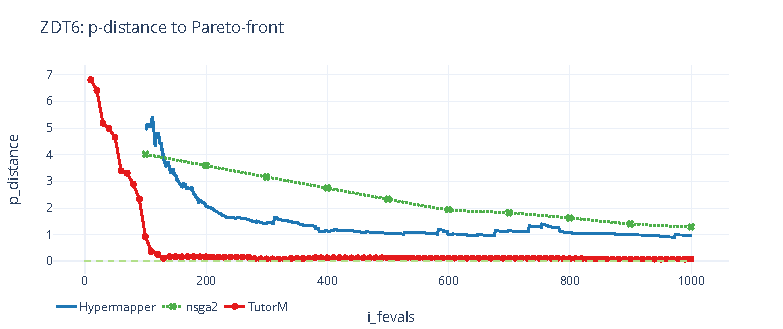
\includegraphics[width=\textwidth]{content/images/zdt6_dist}
                \caption{Average distance of non-dominant solutions to the real Pareto front}
                \label{fig:zdt6_dist}
            \end{subfigure} 
            \begin{subfigure}{0.45\textwidth}
                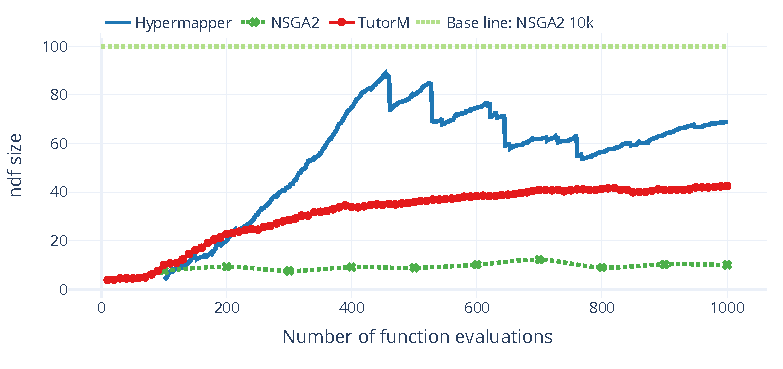
\includegraphics[width=\textwidth]{content/images/zdt6_ndf}
                \caption{Size of non-dominant solutions across the entire set of the measured solutions}
                \label{fig:zdt6_ndf}
            \end{subfigure} 
        \end{subfigure} 

        \begin{subfigure}{\textwidth}
            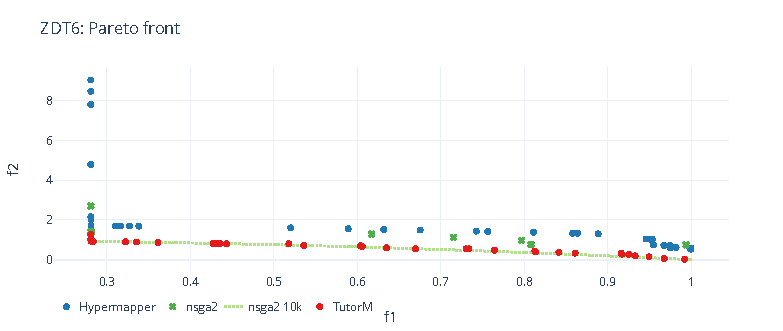
\includegraphics[width=\textwidth]{content/images/zdt6_front}
            \caption{The final assumption of the Pareto optimal solutions (1000 fevals)}
            \label{fig:zdt6_front}
        \end{subfigure} 
        \caption[Comparison of solutions on ZDT6 problem]{A complex comparison of solutions on ZDT6 problem. Final non-dominated points are used to estimate Pareto-optimal solutions.}
        \label{fig:changing_models}    
    \end{figure}


    One of the main advantages of the developed method is the dynamic sampling plan, which depends on the quality of available surrogates. Results show that the number of samples taken from the original plan varies depending on the problem (Figure \ref{fig:changing_models}).
    When samples are enough, several models could periodically swap as best available. It can also be noted that with increasing the sample set, the models give more stable results, and changes become less frequent. In the case of WFG1 problem(\ref{fig:wfg1_models_60}) best accuracy for non-dominated point gave the compositional model with Gradient Boosting Regressor for each objective. In WFG problem, the same compositional model goes ahead other models in the portfolio, but after samples size increased, multi-objective the Gaussian Process Regressor was on the top.
    % === TutorM: surrogate portfolio in action
    \begin{figure}
        \centering
        \begin{subfigure}{\textwidth}
            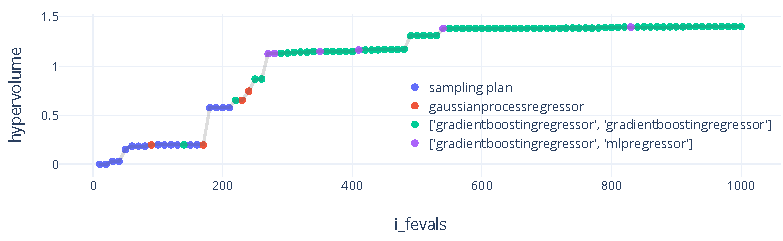
\includegraphics[width=\textwidth]{content/images/dtlz4_models}
            \caption{DTLZ4: sampling plan to the 210th configuration}
            \label{fig:dtlz4_models_210}
        \end{subfigure}
        % \hfill
        
        \begin{subfigure}{\textwidth}
            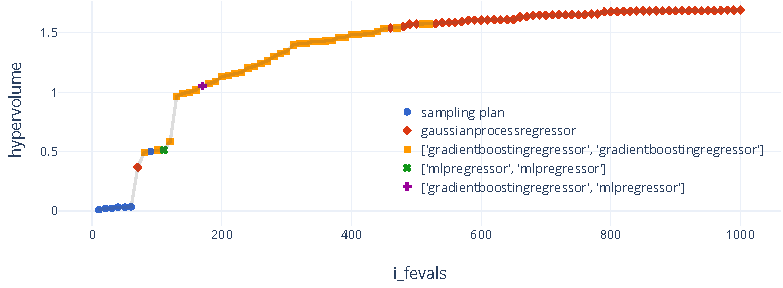
\includegraphics[width=\textwidth]{content/images/wfg1_models}
            \caption{WFG1: sampling plan to the 60th configuration}
            \label{fig:wfg1_models_60}
        \end{subfigure} 

        \caption[Optimization process with dynamic sampling plan and surrogate portfolio.]{Optimization process with dynamic sampling plan and surrogate portfolio. Plots are shown in which step sampling plan was used or which model gives the best accuracy on the test set.}
        \label{fig:changing_models}    
    \end{figure}


    For a satisfactory result, the surrogate model needs to describe the overall landscape and the optimization target area. Figure \ref{fig:wfg_14} shows an example of a case where TutorM produces a better or identical result than an optimal solution. The characteristic of this optimization problem lay in flat landscape regions and relative significance of different parameters that significantly impairs the convergence to the global Pareto-optimal solutions. Hypermapper increase count of non-dominated points, regardless it is local optimum and most samples stack in a small region. NSGA2 after 1000 function evaluations also have high-density regions which could be improved with spending more effort to evaluations. The TutorM found several dozen of Pareto-optimal points, that significantly outperforms Hypermapper and even NSGA2 with 10k evaluations. 
    From WFG4 use case, all over all approaches gain near-optimal results (Fig.\ref{fig:wfg4_front}), but significant advantage over TutorM as it provides an extensive set of solutions (Fig.\ref{fig:wfg4_ndf}) that are well distributed at the Pareto front. As you can see from the graph that the size of the solution increases linearly, which means that effort is spent on improving distribution of the Pareto Pare optimal solutions.


    % As shown in Figure \ref{fig:wfg_14}, TutorM could also outperform the MOEA baseline in 10k evaluations(\ref{sub@fig:wfg1_front}). WFG1 has flat landscape regions hence the convergence of genetic algorithms significantly deteriorates. Hypermapper increase count of non-dominated points, regardless it is local optimum and most samples stack in a small region. Nsga2 after 1000 function evaluations also have high-density regions which could be improved with spending more effort to evaluations. The TutorM has several dozen of Pareto-optimal points from all over the budget, that significantly outperforms Hypermapper and nsga2 even with 10k evaluations. 
    % From WFG4 use case, all over all approaches gain near-optimal results(\ref{fig:wfg4_front}), but significant advantage over TutorM as it provides an extensive set of points(\ref{fig:wfg4_ndf}) that are well distributed at the Pareto front.


    % === WFG1 and WFG4
    \begin{figure}
        \centering
        \begin{subfigure}{\textwidth}
            \begin{subfigure}{0.5\textwidth}
                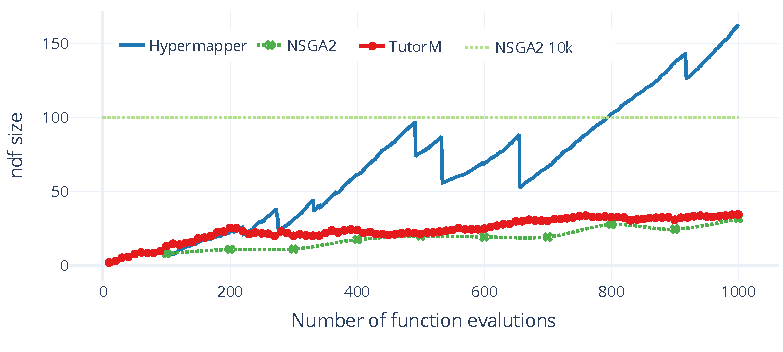
\includegraphics[width=\textwidth]{content/images/wfg1_ndf}
                \caption{WFG1: Size of a non-dominated subset of an evaluated examples}
                \label{fig:wfg1_ndf}
            \end{subfigure} 
            \begin{subfigure}{0.5\textwidth}
                \includegraphics[width=\textwidth]{content/images/wfg1_front}
                \caption{WFG1: Pareto-front approximation}
                \label{fig:wfg1_front}
            \end{subfigure} 
        \end{subfigure} 
        \begin{subfigure}{\textwidth}
            \begin{subfigure}{0.5\textwidth}
                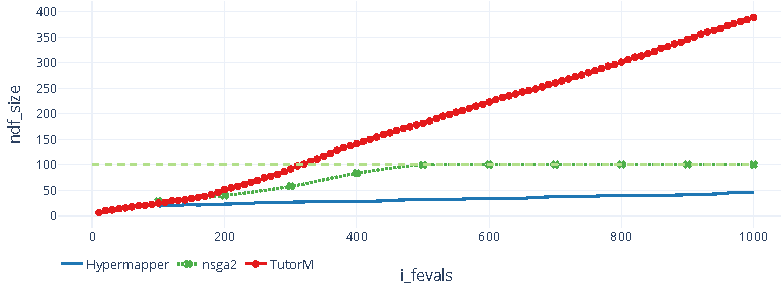
\includegraphics[width=\textwidth]{content/images/wfg4_ndf}
                \caption{WFG4: Size of a non-dominated subset of an evaluated examples}
                \label{fig:wfg4_ndf}
            \end{subfigure} 
            \begin{subfigure}{0.5\textwidth}
                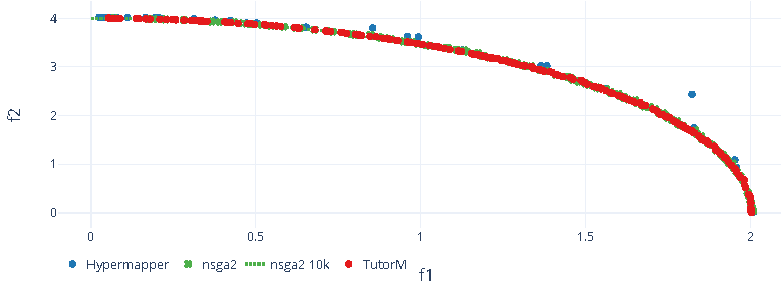
\includegraphics[width=\textwidth]{content/images/wfg4_front}
                \caption{WFG4: Pareto-front approximation}
                \label{fig:wfg4_front}
            \end{subfigure}
        \end{subfigure} 
        \caption[Comparison of solutions on ZDT6 problem]{A complex comparison of solutions on ZDT6 problem. Final non-dominated points are used to estimate Pareto-optimal solutions.}
        \label{fig:wfg_14}    
    \end{figure}


    In this benchmark, we checked all 21 problems from 3 datasets. We considered them as bi-objective with two or three parameters. In all cases, TutorM is ahead of Nypermapper 2.0, and in most cases, TutorM is nearing the baseline solution from NSGA2 with 10k evaluations. The table \ref{tab:magic_five} shows some solutions to the 5 problems. The full list of results is provided in the appendix.
 
        % Please add the following required packages to your document preamble:
    % \usepackage{booktabs}
    % \usepackage{multirow}
    \begin{table}[]
        \centering
        \caption{Comparison of final results after 1000 function evaluations}
        \begin{tabular}{@{}lllllll@{}}
        \toprule
                                                                                                & Metric        & ZDT4             & ZDT6             & DTLZ4             & WFG1             & WFG4             \\ \midrule
        \multirow{4}{*}{\textbf{TutorM}}                                                          & Hypervolume   & \textbf{99,80\%} & \textbf{99,43\%} & \textbf{99,829\%} & \textbf{95,75\%} & \textbf{99,28\%} \\ \cmidrule(l){2-7} 
                                                                                                & p-distance    & \textbf{0,01}    & \textbf{0,09}    & \textbf{0,001}    & -                & -                \\ \cmidrule(l){2-7} 
                                                                                                & ndf-size      & \textbf{50,0\%}  & 4,26\%           & 0,2\%             & 3,44\%           & \textbf{38,90\%} \\ \cmidrule(l){2-7} 
                                                                                                & space-metric  & \textbf{0,78}    & 0,17             & 0,666             & 0,51             & \textbf{1}       \\ \midrule
        \multirow{4}{*}{\textbf{NSGA2}}                                                           & Hypervolume   & 83,43\%          & 83,84\%          & 87,807\%          & 30,52\%          & 83,95\%          \\ \cmidrule(l){2-7} 
                                                                                                & p-distance    & 0,04             & 1,29             & 0,002             & -                & -                \\ \cmidrule(l){2-7} 
                                                                                                & ndf-size      & 8,77\%           & 1,01\%           & 9,600\%           & 3,18\%           & 10\%             \\ \cmidrule(l){2-7} 
                                                                                                & space-metric  & 0,19             & 0,04             & 0,323             & 0,28             & 0,58             \\ \midrule
        \multirow{4}{*}{\textbf{Hypermaper}}                                                      & Hypervolume   & 97,32\%          & 82,86\%          & 64,57\%           & 44,12\%          & 84,39\%          \\ \cmidrule(l){2-7} 
                                                                                                & p-distance    & 0,90             & 1,12             & 0,059             & -                & -                \\ \cmidrule(l){2-7} 
                                                                                                & ndf-size      & 5,42\%           & \textbf{6,25\%}  & 1,177\%           & \textbf{10,24\%} & 3,26\%           \\ \cmidrule(l){2-7} 
                                                                                                & space-metrics & 0,11             & 0,08             & 0,029             & 0,31             & 0,06             \\ \midrule
        \multirow{4}{*}{\textbf{\begin{tabular}[c]{@{}l@{}}NSGA2 50k\\ (Base line)\end{tabular}}} & Hypervolume   & 100\%            & 100\%            & 100\%             & 100\%            & 100\%            \\ \cmidrule(l){2-7} 
                                                                                                & p-distance    & 2,04e-05         & 0,0003           & 8,81e-06          & -                & -                \\ \cmidrule(l){2-7} 
                                                                                                & ndf-size      & 0,72\%           & 0,72\%           & 0,360\%           & 0,72\%           & 0,72\%           \\ \cmidrule(l){2-7} 
                                                                                                & space-metric  & 1                & 1                & 1                 & 1                & 0,60             \\ \bottomrule
        \end{tabular}
        \label{tab:magic_five}
    \end{table}




        % \begin{table}[]
    %     \centering
    %     \caption{Comparison of final results after 1000 feature evaluations}
    %     \resizebox{\textwidth}{!}{%
    %     \begin{tabular}{@{}ccccccc@{}}
    %     \toprule
    %                                          & \textbf{Metric}        & \textbf{ZDT4} & \textbf{ZDT6} & \textbf{DTLZ4} & \textbf{WFG1} & \textbf{WFG4} \\ \midrule
    %     \multirow{4}{*}{\textbf{TutorM}}     & \textbf{hypervolume}   & 99,45\%       & 99,01\%       & 99,27\%        & 115,60\%      & 95,95\%       \\
    %                                          & \textbf{p-distance}    & 1,336         & 0,522         & 0,022          & -             & -             \\
    %                                          & \textbf{ndf-size}      & 183,022       & 31,528        & 119,308        & 24,158        & 183,244       \\
    %                                          & \textbf{space-metrics} & 0,103         & 0,142         & 0,186          & 0,129         & 0,032         \\ \midrule
    %     \multirow{4}{*}{\textbf{NSGA2}}      & \textbf{hypervolume}   & 97,57\%       & 87,46\%       & 95,87\%        & 45,01\%       & 91,87\%       \\
    %                                          & \textbf{p-distance}    & 1,391         & 1,872         & 0,022          & -             & -             \\
    %                                          & \textbf{ndf-size}      & 44,000        & 11,455        & 39,900         & 20,164        & 82,436        \\
    %                                          & \textbf{space-metrics} & 0,176         & 0,355         & 0,268          & 0,228         & 0,038         \\ \midrule
    %     \multirow{4}{*}{\textbf{Hypermaper}} & \textbf{hypervolume}   & 96,82\%       & 66,95\%       & 81,29\%        & 40,66\%       & 74,09\%       \\
    %                                          & \textbf{p-distance}    & 2,024         & 1,850         & 0,076          & -             & -             \\
    %                                          & \textbf{ndf-size}      & 28,908        & 52,746        & 10,743         & 81,512        & 30,158        \\
    %                                          & \textbf{space-metrics} & 0,1386        & 0,11621       & 0,5282         & 0,0870        & 0,1032        \\ \midrule
    %     \multirow{4}{*}{\textbf{\begin{tabular}[c]{@{}c@{}}NSGA2\\ 10k eval\end{tabular}}} & \textbf{hypervolume}      & 100,00\% & 100,00\% & 100,00\% & 100,00\% & 100,00\% \\
    %                                          & \textbf{p-distance}    & 0,152         & 0,256         & 0,002          & -             & -             \\
    %                                          & \textbf{ndf-size}      & 93,901        & 79,776        & 93,990         & 85,196        & 98,087        \\
    %                                          & \textbf{space-metrics} & 0,033         & 0,074         & 0,039          & 0,051         & 0,016         \\ \bottomrule
    %     \end{tabular}%
    %     }
    % \label{tab:magic_five} 
    % \end{table}

% --------------------------------------------------------------------------------------------
% ---------------------       Benchmark 2: Dynamic sampling plan and parameter selection
% --------------------------------------------------------------------------------------------
\section{Benchmark 2: Inner parameters}
    This benchmark examines the effect of internal parameters on the performance and quality of optimization.It is necessary to determine which parameters for model-based optimization are crucial.

    \subsection{TutorM parameters}
    In addition to the common model-based parameters, it is necessary to investigate the impact of additional TutorM parameters such as validation thresholds, test set size and prediction size. Unfortunately, there is not enough information about how to configure the model-based parameter optimization  \cite{}. Conducting such analysis will be useful not only for the availability of the TutorM but also for the general tuning of model-based optimization. 
    Due to limited time, we consider only the ZDT4 and ZDT6 problems with a surrogate portfolio from the previous benchmark, but without the Gaussian regression model. 


    The following parameters are highlighted in the developed TutorM class:
    \begin{itemize}
        \item \textbf{Initial dataset} [0, 100, 500, 750]. The initial number of measured points from the search space. At the same time, the total budget for measurements remains unchanged and equals 1000.
        \item Surrogate validation. Criteria and parameters for evaluating the usefulness of the surrogate model.
            \begin{itemize}
                \item \textbf{Train/test split} [75/25, 90/10] train and test samples split
                \item \textbf{Cross-Validation threshold}[0.2, 0.65, 0.9] minimum accuracy threshold for any round in cross-validation.
                \item \textbf{Test threshold} [0, 0.6, 0.9] minimum accuracy threshold on the test set.
            \end{itemize}
        \item \textbf{Optimization search algorithm} [NSGA2, MOEA-Ctrl] optimization algorithm for multi-objective solutions. 
        \item \textbf{Solution combinations} [Non-dominated front score, Stacking] approach for choosing a set of solutions from a valid surrogate model. Since several models can be valid and each one provides its own set of decisions, we have to choose which one to pick. \emph{Non-dominated front score (ndf score)} prefers the surrogate model with the highest precision for non-dominant solutions, whereas the \emph{stack} integrates all available surrogate solutions into one set of solutions. 
        \item \textbf{Prediction count} [10, 100] number of random solutions for a real evaluation that are selected from the set of solutions.
    \end{itemize}

    As a result of the full factorial design, 576 possible combinations were obtained. Each combination was repeated 5 times and averaged. Conclusions were made on the selected 40 best and worst combinations.

    % -- ZDT6
    First, let's consider the ZDT6 problem. Considering the figure \ref{fig:conf_zdt6}, it can be observed that the most significant impact on the result made by the combination of solution. There is a clear advantage in combining solutions into a stack. The second important parameter is the optimization algorithm (Solver). Best configurations prefer to include a combination of Genetic Algorithms (MOEA-Ctrl) as optimization solver.

    Let's look at these options in more detail (Fig. \ref{fig:conf_zdt6_sign}). The impact of changing the optimization solver is highly dependent on the solution combination strategy. Improvement in result for MOEA-Ctrl solver is more significant when their results are combined into a stack.

    This advantage can be explained by the fact that the stack reduces the bias of surrogate models while the combination of genetic algorithms decreases prediction variance.

    % -- ZDT4
    Now let's look at the ZDT4 problem (Fig. \ref{fig:conf_zdt4}). The results are similar to those obtained with the ZDT6 problem: the solutions stack take part almost in all best configurations. However, in this problem, there is no clear dominance of an optimization solver, but there is an impact on results from the validation thresholds (Fig. \ref{fig:conf_zdt4_sign}). 

    A significant difference is available for the cross-validation threshold in the case of 'ndf' solutions' set (Fig. \ref{fig:conf_zdt4_worst}). For example, a harmful validation threshold could have a division of results into two parts: the upper one was obtained from the sampling plan because the models did not pass validation; the lower one corresponds to the cases when a valid model is finally available and guide an optimization process. It should be noted that the stack of solutions does not have such a separation that is related to the general characteristics of this technique to reduce the solution's bias.
    
    Another fascinating conclusion could be done from the initial sample size.The worst and the best configurations are most affected by the low or missing sampling plan. Reason for this is that the small number of samples may lead to a surrogate model fallacy while, at the same time, the small number of samples provide more opportunities for optimization search. So, this is confirmation of the importance of the dynamic sampling plan.

    % ===  ------------------------------------- ZDT6
    \begin{figure}
        \centering
        \begin{subfigure}{\textwidth}
            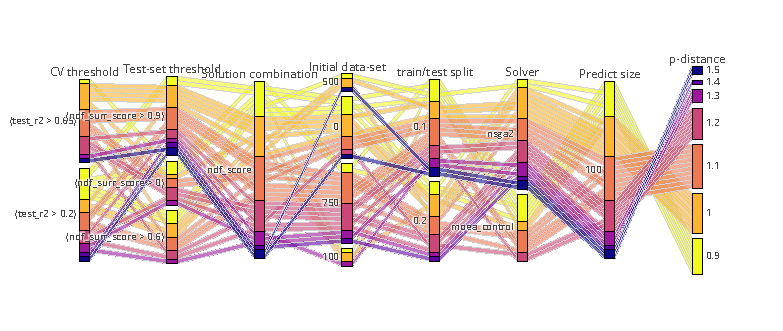
\includegraphics[width=\textwidth]{content/images/conf_zdt6_worst}
            \caption{40 worst configurations}
            \label{fig:conf_zdt6_worst}
        \end{subfigure} 
        % \hfill
        
        \begin{subfigure}{\textwidth}
            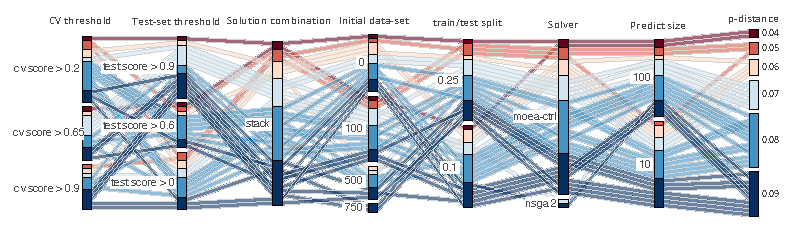
\includegraphics[width=\textwidth]{content/images/conf_zdt6_best}
            \caption{40 best configurations}
            \label{fig:conf_zdt6_best}
        \end{subfigure} 

        \caption[ZDT6: The selection from average result of best and worst configurations.]{ZDT6: The selection from average result of best and worst configurations.}
        \label{fig:conf_zdt6}    
    \end{figure}

    % === ZDT 6
    \begin{figure}
        \centering

        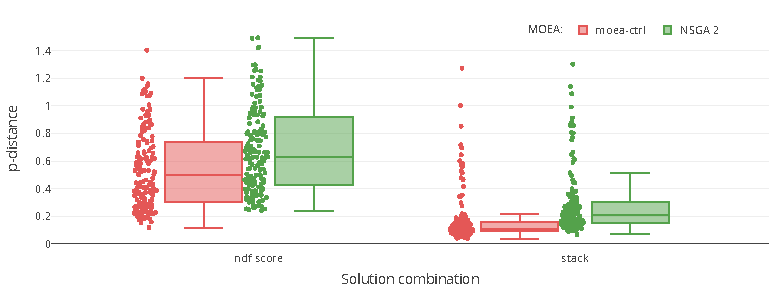
\includegraphics[width=0.8\textwidth]{content/images/conf_zdt6_solver}

        \caption[Correlation between the most influenceable parameters for the ZDT6]{Correlation between the most influenceable parameters for the ZDT6: solution combination strategy and optimization algorithm}
        \label{fig:conf_zdt6_sign}    
    \end{figure}


    % === -------------------------------------- ZDT 4
    \begin{figure}
        \centering
        \begin{subfigure}{\textwidth}
            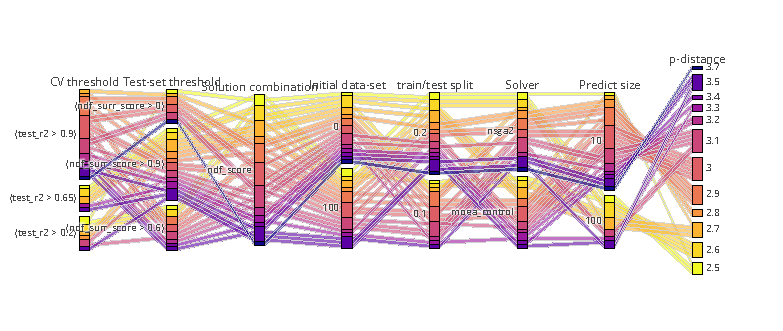
\includegraphics[width=\textwidth]{content/images/conf_zdt4_worst}
            \caption{ZDT4: worst configurations}
            \label{fig:conf_zdt4_worst}
        \end{subfigure} 
        \hfill
        
        \begin{subfigure}{\textwidth}
            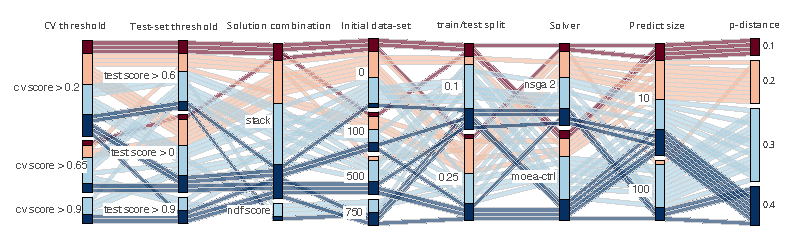
\includegraphics[width=\textwidth]{content/images/conf_zdt4_best}
            \caption{ZDT4: best configurations}
            \label{fig:conf_zdt4_best}
        \end{subfigure} 

        \caption[ZDT4: The selection from average result of best and worst configurations.]{ZDT4: The selection from average result of best and worst configurations.}
        \label{fig:conf_zdt4}    
    \end{figure}

    % === ZDT4
    \begin{figure}
        \centering
        \begin{subfigure}{\textwidth}
            \begin{subfigure}{0.45\textwidth}
                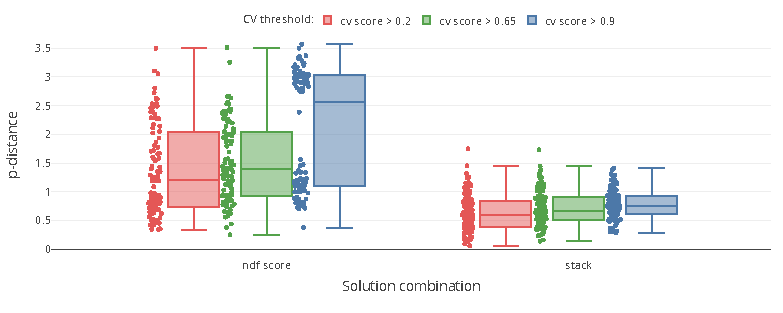
\includegraphics[width=\textwidth]{content/images/conf_zdt4_cv_score}
                \caption{An impact of the cross-validation's threshold}
                \label{fig:zdt4_pred_solver}
            \end{subfigure} 
            \begin{subfigure}{0.45\textwidth}
                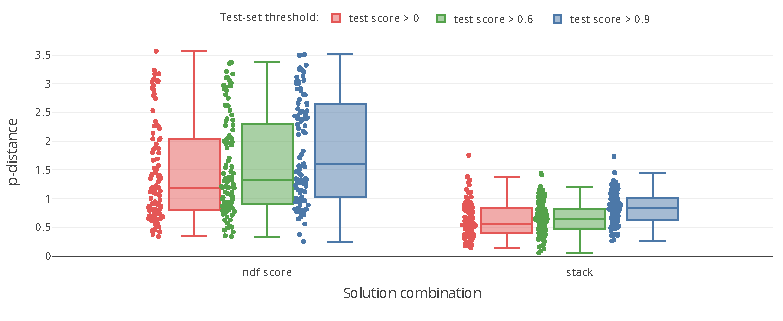
\includegraphics[width=\textwidth]{content/images/conf_zdt4_test_score}
                \caption{An impact of the test-set-validation's threshold}
                \label{fig:zdt4_comb_valid}
            \end{subfigure}
        \end{subfigure}


        \caption[Correlation between the most influenceable parameters for the ZDT4]{Correlation between the most influenceable parameters for the ZDT4} 
        \label{fig:conf_zdt4_sign}    
    \end{figure}

    % ====================================================== Start set for Hypermapper 2.0
    \subsection{Sampling plan size}
    Purpose of this experiment is to review the dependencies between the optimization result and the sampling plan size. The HyperMapper was selected as a foundation for analysis because it has a static implementation of the optimization algorithm with the surrogate model.

    The results are shown in the following figure \ref{fig:hmapper_start_set}. 
    For WFG1 and WFG4 problem, the criterion is the hypervolume and for ZDT4 and ZDT6 problem is the p-distance. Of all the results, the initial sampling plan is the least effects to the WFG6. Since this problem is unimodal and is described merely by fewer samples, other problems have a more complicated multimodal landscape that shown by unstable results. It is noticeable that the plan depends on the problem type. The optimization result may deteriorate which caused by increasing or decreasing the number of samples.

    \begin{figure}
        \centering
        \begin{subfigure}{\textwidth}
            \begin{subfigure}{0.45\textwidth}
                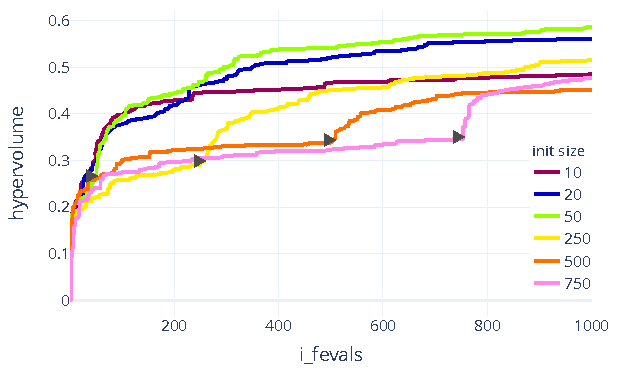
\includegraphics[width=\textwidth]{content/images/hypermapper_wfg1_start_set}
                \caption{WFG1}
                \label{fig:hmapper_wfg1_start_set}
            \end{subfigure}
            \begin{subfigure}{0.45\textwidth}
                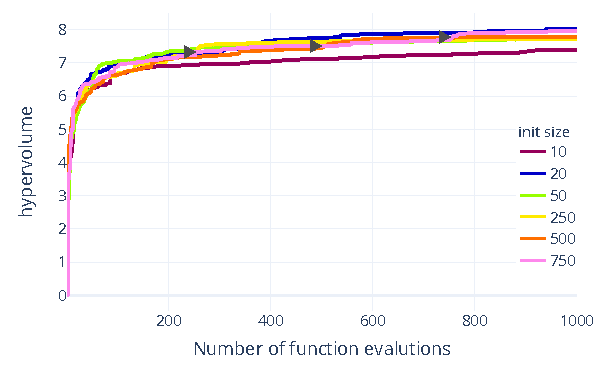
\includegraphics[width=\textwidth]{content/images/hypermapper_wfg4_start_set}
                \caption{WFG4}
                \label{fig:hmapper_wfg4_start_set}
            \end{subfigure}
        \end{subfigure} 
        \hfill

        
        \begin{subfigure}{\textwidth}
            \begin{subfigure}{0.45\textwidth}
                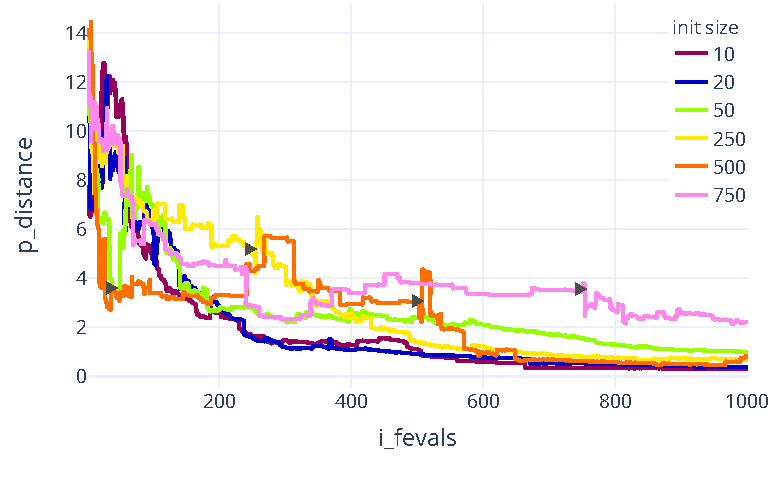
\includegraphics[width=\textwidth]{content/images/hypermapper_zdt4_start_set}
                \caption{ZDT4}
                \label{fig:hmapper_zdt4_start_set}
            \end{subfigure}
            \begin{subfigure}{0.45\textwidth}
                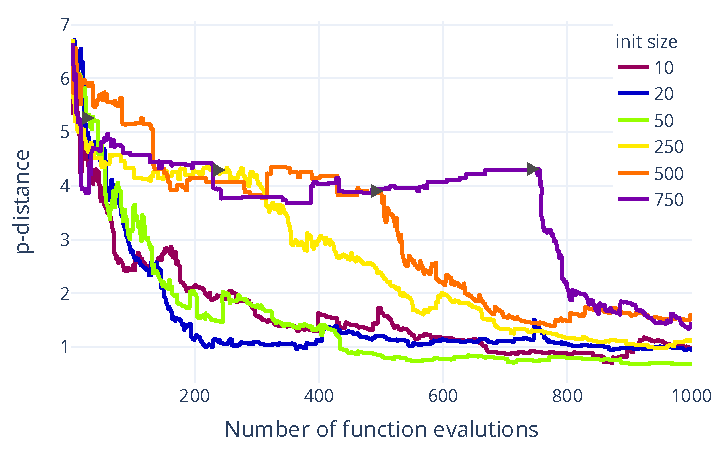
\includegraphics[width=\textwidth]{content/images/hypermapper_zdt6_start_set}
                \caption{ZDT6}
                \label{fig:hmapper_zdt6_start_set}
            \end{subfigure}
        \end{subfigure} 

        \caption[Influence of the initial sample plan for optimization with Hypermapper 2.0.]{Influence of the initial sample plan for optimization with Hypermapper 2.0.}
        \label{fig:hmapper_start_set}    
    \end{figure}



% --------------------------------------------------------------------------------------------
% ---------------------       Benchmark 3: Many-objective optimization, scaling
% --------------------------------------------------------------------------------------------
\section{Benchmark 3: Scalability of surrogate models. RQ1.1}
    Not only the type of the problem landscape but also its dimensions is an essential factor for picking the surrogate model. The advantage of a surrogate model might be lost when the number of optimization parameters or criteria are changed. The goal of this experiment is to find out the scalability of surrogate models. 


    The following surrogates were selected for verification:
    \begin{itemize}
        \item \emph{Gaussian Process Regressor} with kernel design from GPML\cite{RasmussenN10}. Gaussian process models are well known as commonly used in Bayesian optimization for a wide variety of problems. 
        \item MLPRegressor is a \emph{neural network} implementation from the \textit{sklearn} framework. Neural networks could automatically discover useful representations in high-dimensional data by learning multiple layers \cite{WilsonHSX16}. Because this model simultaneously extrapolates all objectives, we intuitively chose an architecture that consists of 5 layers and 100 neurons per layer.
        \item The surrogate portfolio is included of Gradient Boosting Regressor and \emph{SVR (RBF kernel)} as in the mentioned benchmark number 2. Also, a neural network with 5 cells and 50 neurons per layer was added. For the sake of the experiment, all models in the portfolio are composite and can be dynamically combined depending on the validation results. The surrogate portfolio is included of the Gradient Boosting Regressor and the SVR (RBF kernel). Also, a neural network with 5 layers and 50 neurons per layer was added. All models in the portfolio are composite and can be dynamically combined depending on the validation results.
    \end{itemize}

    For evaluation scalability property for the surrogate models, \emph{DTLZ2} problem was selected. It is unimodal problem with multiple global optima and concave geometry of the Pareto front. During the experiment, the number of optimization criteria changes with a constant number of parameters. For all cases, the experiment was repeated 5 times. The figure \ref{fig:scale_dtlz2} shows the three selected surrogate strategies with metrics of the average distance to the Pareto front (top line) and a time spent per complete an optimization iteration (bottom line). Note that the Gaussian model shows significantly better results relative to other approaches but only for the bi-objective problem. Increasing the criteria to 4, converging to a solution is only available for the neural network and portfolio. At the same time, the Gaussian model becomes incorrect and begins to increase the time required to build exponentially.
    
    There is also an open question as to which parameters to choose for the surrogate model. The suitability and quality of the surrogate are highly dependent on the parameters (number of layers, type of core). In turn, for the surrogate portfolio, the parameters determine how to build and select surrogate models. The same model but with different parameters, is evaluated in the portfolio as separate entities. It is a great advantage to apply a dynamic and scalable approach that can adapt to a specific problem. This is the answer to \hyperref[RQ1.1]{RQ1.1}.

    
    Hence, the necessary criterion for scaling surrogates is not just the choice of one model for all cases, but the dynamic combination of the strong properties of several models to achieve better results with limited resources.


    \begin{figure}
        \centering
        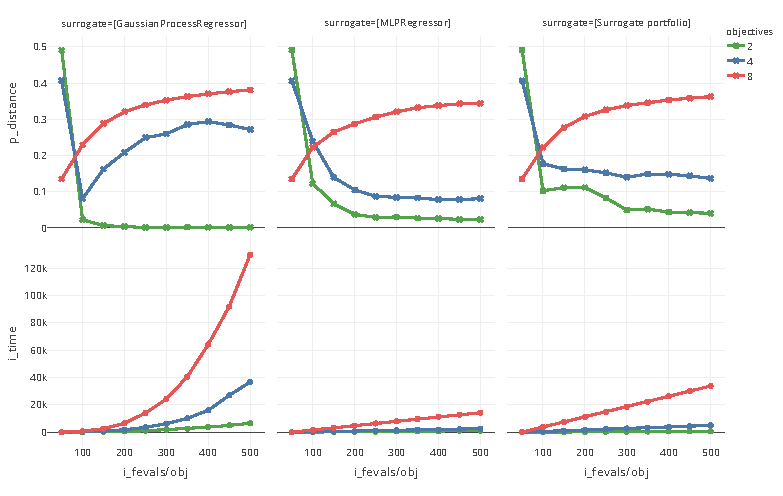
\includegraphics[width=\textwidth]{content/images/scale_dtlz2}
        \caption[Scaling example for the three variants of the surrogate on the DTLZ2.]{Scaling example for the three variants of the surrogate on the DTLZ2. Scaling example for the three variants of the surrogate on the DTLZ2  with the 9-dimensional objective space.}
        \label{fig:scale_dtlz2}    
    \end{figure}



    % 

    % Objectives: 1) detect iterative improvement, a convergence of the primary metric 2) time for evaluation

    % Usecases: GausianModel, GausianModel + Gradient, GausianModel + random forest, 

    % Scale: objectives - 2,4,8,10; params - 2,4,8,10

    % ! [ Hypermapper baseline; X - objectives Y - p-distance/time]




% --------------------------------------------------------------------------------------------
% ------------------------------------------------     Discussion 
% --------------------------------------------------------------------------------------------
\section{Discussion}

Up to now, most papers used the The quality of the results obtained with X was similar to the results obtained with Y, but with significantly fewer exactly evaluated solutions during the optimization process. 


% consume an inordinate amount of time.


The purpose of this work is to explore the possibility of using single-objective models for many-objective optimizations. To accomplish this goal, the composite model has been implemented. It is used to combine models into a portfolio and dynamically select them. Furthermore, the stepwise validation approach has been adapted to evaluate the usability of the surrogate model.

% Discussion

% non-separable
% or have a deceptive fitness landscape

% However, GAs, or at least some variants of them, are not 100'\%' ruled out.

% +’, ’−’ and ’≈’, which indicate that the result is significantly better, significantly worst and statistically similar to the result in the control column, respectively. 


% On the left side the learning curve of a naive Bayes classifier is shown for the digits dataset. Note that the training score and the cross-validation score are both not very good at the end. However, the shape of the curve can be found in more complex datasets very often: the training score is very high at the beginning and decreases and the cross-validation score is very low at the beginning and increases. On the right side we see the learning curve of an SVM with RBF kernel. We can see clearly that the training score is still around the maximum and the validation score could be increased with more training samples.
% https://scikit-learn.org/0.15/auto_examples/plot_learning_curve.html




% Compared to Auto-WEKA, this is much more data-efficient: in
% Auto-WEKA, evaluating the performance of an ensemble with 5 components requires the construction
% and evaluation of 5 models; in contrast, in auto-sklearn, ensembles come largely for free, and it is
% possible to mix and match models evaluated at arbitrary times during the optimization.


% This makes the archive gradually move towards the Pareto-front.
% 80% of the computing-time is spent in the area close to the Pareto front.


% We would like to prove that the use of hierarchical surrogates has a higher probability to find the optimum of the optimization problem in Eq. (4) ref[Evolutionary optimization with hierarchical surrogates]


% Test problems ZDT1, ZDT2, and ZDT3 show a different trend in function evaluations as compared to OSY.


% In contrast to PR, ANN, RBF, GP, Ranking SVM is invariant to

% The measurements were performed on an Intel Core i7-8700CPU machine with 64G of memory using Fedora Server 29.












    % The first benchmark presented a subset of the problems listed in Table \ref{bench_problems}. They have a wide range of properties which should give a notion of how the optimization strategy works.
    % % ==== multi-objective test problems
    % \begin{table}[]
    %     \centering
    %     \resizebox{\textwidth}{!}{%
    %         \begin{tabular}{@{}cccccc@{}}
    %         \toprule
    %         \multirow{2}{*}{\textbf{Problem}} &
    %         \multirow{2}{*}{\textbf{Objective}} &
    %         \multirow{2}{*}{\textbf{Modality}} &
    %         \multirow{2}{*}{\textbf{Geometry}} &
    %         \multicolumn{2}{c}{\textbf{Landscape}} \\ \cmidrule(l){5-6}
    %                     &                 &                      &               & \textbf{Bias}    & \textbf{\begin{tabular}[c]{@{}c@{}}Many-to-one \\ mappings\end{tabular}} \\ \midrule
    %         \textbf{ZDT4}  & bi-objective    & unimodal, multimodal & convex        & -                & -                                                                        \\
    %         \textbf{ZDT6}  & bi-objective    & multimodal           & concave       & +                & +                                                                        \\
    %         \textbf{DTLZ4} & multi-objective & unimodal             & concave       & +                & +                                                                        \\
    %         \textbf{WFG1}  & multi-objective & unimodal             & convex, mixed & polynomial, flat & +                                                                        \\
    %         \textbf{WFG4}  & multi-objective & multimodal           & concave       & -                & +                                                                       \\ \bottomrule
    %         \end{tabular}%
    %     }
    %     \caption{Selected multi-objective test problems}
    %     \label{bench_problems}
    % \end{table}
    \chapter{Future Work}\label{sec:future_work}

The developed strategy in this thesis has a component structure and a unified interface. All major components are easily replaceable and scalable. A strong feature of our solution is the adaptation of optimization to a scaled unknown problem. That is why further integration with the \emph{software product line} is a promising improvement. A right solution for this is to choose \hyperref[alg:BRISE]{BRISE} - software product line for parameter tuning. It has the necessary key features such as stop criterion, noisy experiments and distributed architecture. The integration of this thesis into the BRISE will improve its variability and scalability.

There are other several directions that the project aims to focus on in future improvement. 
\begin{itemize}
    \item Promising results have been obtained for the combination of optimization techniques with surrogate modes. Further investigation in extensive parallel combination \emph{surrogate models and optimization algorithms} could significantly improve optimization results.
    \item It is advisable to change the composition of the portfolio to discard those models that are performing poorly. This \emph{dynamic models collection} for the surrogate portfolio could improve the exploration of new models and reduce additional time costs.
\end{itemize}











\chapter{Conclusion}\label{sec:conclusion}

    In this thesis, we propose a strategy for dynamic composition of surrogate models which allows using the surrogate portfolio for tuning black-box function.
        Our investigation revealed that the current surrogate-based optimization operates with a single type of models or static combination of several varieties. These approaches lack variability and cannot be adapted for an arbitrary problem. Our research goal was to decompose the model-based multi-objective optimization to reusable and comparable components. 
    To achieve this goal was made following research contributions:
    \begin{enumerate}
        \item At first, we developed the compositional model for an arbitrary type of surrogate model. We established and implemented a component that combined several models into one surrogate hypothesis. Nevertheless, for an arbitrary, unknown problem, dynamic integration of surrogates into a composite model is required.
        \item Next, we adapted the cross-validation technique to validate and compare surrogate models. A multi-step validation is essential to avoid the model underfeed and overfeed. Validation information enables dynamically decide on picking the right models or use the sampling plan as a default variant.
        \item Eventually, we implemented a surrogate portfolio that combines functionality from the preceding paragraphs. The portfolio allows select and combines multiple surrogate models dynamically concerning a concrete problem. This property means that a portfolio can offer more than one surrogate hypothesis for optimization.
        \item In the end, we improved the variability and extensibility not only for surrogate models but also for optimization algorithms. For example, this is the possibility to combine solutions into a stack to reduce overall error.
    \end{enumerate}


    Combining all these contributions enabled us to achieve excellent results in a wide range of optimization tasks. For almost all problems, our approach has demonstrated a significant advantage over all solution criteria. The analysis of the parameters showed that the most significant influence is obtained from the solution combination (assumptions about the Pareto front). We have implemented the dynamic sampling plan which is to select additional random points if there is no valid model. This strategy  improved the result as the exploration-exploitation balance is determined for each optimization problem independently.
    Next crucial issue is the optimization of multidimensional space. We have shown that a surrogate model can be applied to a small number of objectives but not be inappropriate if the objectives are increased. The optimal solution for this may be a flexible combination of better models at each optimization iteration.

    We consider that the results accomplished in this thesis can be useful for improving the parameter tuning and for the overall model-based optimization.

    % \section{Future Work}
    %     \paragraph{Prior knowledge. Transfer learning}
    %      What is already implemented and how it could be improved.
    %      \begin{itemize}
    %          \item Model portfolio selection and combination.
    %          \item Prior distribution of parameters. Bayesian kernels.
    %          \item Human in the loop. Reducing the search space.
    %      \end{itemize}

    % Further work will consider h(θ) as yet another expensive noisy black-box function, and the use of a CMA-ES in the hyper-parameter space will be studied.


    % \section{General Conclusion}
        %  \paragraph{BRISE}
        %  Modelbase line in parameter tuning for software Product Line for Parameter Tuning




        %  In surrogate-assisted evolutionary search, the choice of surrogate modeling technique can highly affect the performance of the search. To address this issue, we proposed a novel strategy in this paper to do surrogate


        %  There are several directions that the project aims to focus on in future development. 












%  We expect that our results would similarly generalize to these.
    
    \bibliographystyle{alpha}
    \bibliography{content/bibliography.bib}

    % must be invoked for correct page numbering in the appendix and all lists
    \backmatter
    

    \appendix
    
    \chapter{Appendix}
        \section{Additional Information}
            % ======= SUMMARY DTLZ
            % Please add the following required packages to your document preamble:
% \usepackage{booktabs}
% \usepackage{multirow}
% \usepackage{graphicx}
\begin{table}[]
    \centering
    \label{tab:dtlz_summary}
    \resizebox{\textwidth}{!}{%
    \begin{tabular}{@{}llllll@{}}
    \toprule
    \textbf{Problem}                & \textbf{Approach}        & $\downarrow$ \textbf{p-distance} & $\uparrow$ \textbf{Hypervolume} \%  & $\uparrow$ \textbf{ndf size} \% & $\uparrow$  \textbf{ndf space} \\ \midrule
    \multirow{4}{*}{DTLZ1} & Base line       & 0,800           & 100             & 0,24           & 1     \\ \cmidrule(l){2-6} 
    & NSGA2 1k        & \textbf{3,277}  & 56,577          & \textbf{1,56}  & 0,046 \\ \cmidrule(l){2-6} 
    & TutorM          & 51,611          & \textbf{98,163} & 0,54           & 0,058 \\ \cmidrule(l){2-6} 
    & Hypermapper 2.0 & 74,251          & 86,173          & 0,78           & 0,049 \\ \midrule
\multirow{4}{*}{DTLZ2} & Base line       & 5,19e-06        & 98,603          & 0,24           & 0,39 \\ \cmidrule(l){2-6} 
    & TutorM          & \textbf{0,0004} & \textbf{100}    & \textbf{82,56} & 1     \\ \cmidrule(l){2-6} 
    & NSGA2 1k        & 0,003           & 80,415          & 10          & 0,301 \\ \cmidrule(l){2-6} 
    & Hypermapper 2.0 & 0,058           & 76,103          & 2,84           & 0,063 \\ \midrule
\multirow{4}{*}{DTLZ3} & Base line       & 0,4           & 100             & 0,24           & 1     \\ \cmidrule(l){2-6} 
    & NSGA2 1k        & \textbf{4,430}  & 74,937          & 0,82           & 0,037 \\ \cmidrule(l){2-6} 
    & TutorM          & 38,735          & \textbf{97,743} & 0,40           & 0,045 \\ \cmidrule(l){2-6} 
    & Hypermapper 2.0 & 92,228          & 95,010          & 0,70           & 0,047 \\ \midrule
\multirow{4}{*}{DTLZ4} & Base line       & 8,81e-06        & 100             & 0,36           & 1     \\ \cmidrule(l){2-6} 
    & TutorM          & \textbf{0,001}  & \textbf{99,829} & \textbf{30,68} & 0,666 \\ \cmidrule(l){2-6} 
    & NSGA2 1k        & 0,002           & 87,807          & 9,60           & 0,323 \\ \cmidrule(l){2-6} 
    & Hypermapper 2.0 & 0,059           & 64,579          & 1,18           & 0,029 \\ \midrule
\multirow{4}{*}{DTLZ5} & Base line       & 1,62e-05        & 98,631          & 0,24           & 0,486 \\ \cmidrule(l){2-6} 
    & TutorM          & \textbf{0,0004} & \textbf{100}    & \textbf{80,88} & 1     \\ \cmidrule(l){2-6} 
    & NSGA2 1k        & 0,002           & 81,729          & 10          & 0,434 \\ \cmidrule(l){2-6} 
    & Hypermapper 2.0 & 0,058           & 78,463          & 3,02           & 0,06 \\ \midrule
\multirow{4}{*}{DTLZ6} & Base line       & 0,009           & 100             & 0,24           & 1     \\ \cmidrule(l){2-6} 
    & TutorM          & \textbf{0,123}  & \textbf{98,064} & 3,70           & 0,142 \\ \cmidrule(l){2-6} 
    & NSGA2 1k        & 1,011           & 54,258          & 2,88           & 0,128 \\ \cmidrule(l){2-6} 
    & Hypermapper 2.0 & 1,657           & 18,355          & 2,22           & 0,084 \\ \midrule
\multirow{4}{*}{DTLZ7} & Base line       & 2,42e-07        & 99,938          & 0,24           & 0,364 \\ \cmidrule(l){2-6} 
    & TutorM          & \textbf{0,0003} & \textbf{100}    & \textbf{87} & 1     \\ \cmidrule(l){2-6} 
    & NSGA2 1k        & 0,160           & 92,891          & 3,04           & 0,128 \\
    & Hypermapper 2.0 & 0,781           & 91,129          & 2,24           & 0,081 \\ \cmidrule(l){2-6} 
\end{tabular}%
    }
    \caption{DTLZ problem set: Comparison between Hypermapper 2, NSGA2 and TutorM.  All Results were averaged after 5 reps with a 1,000 evaluations budget.
    The general baseline is the NSGA2 with 50k evaluations (100 population size in 500 generations)}
    \end{table}


            % ======= SUMMARY ZDT
            % Please add the following required packages to your document preamble:
% \usepackage{booktabs}
% \usepackage{multirow}
% \usepackage{graphicx}
\begin{table}[]
    \centering
    \resizebox{\textwidth}{!}{%
    \begin{tabular}{@{}llllll@{}}
    \toprule
    \textbf{Problem}                & \textbf{Approach}        & $\downarrow$ \textbf{p-distance} & $\uparrow$ \textbf{Hypervolume} \%  & $\uparrow$ \textbf{ndf size} \% & $\uparrow$  \textbf{ndf space} \\ \midrule
    \multirow{4}{*}{ZDT1} & Base line       & 1,08e-05          & 99,78          & 0,16           & 0,22          \\ \cmidrule(l){2-6} 
                          & TutorM          & \textbf{4,74e-05} & \textbf{100}   & \textbf{90,33} & \textbf{1}    \\ \cmidrule(l){2-6} 
                          & NSGA2 1k        & 0,02              & 89,86          & 9,66           & 0,08          \\ \cmidrule(l){2-6} 
                          & Hypermapper 2.0 & 0,12              & 98,93          & 10,36          & 0,04          \\ \midrule
    \multirow{4}{*}{ZDT2} & Base line       & 1,04e-14          & 99,79          & 0,16           & 0,29          \\ \cmidrule(l){2-6} 
                          & TutorM          & \textbf{0,00013}  & \textbf{100}   & \textbf{86,87} & \textbf{1}    \\ \cmidrule(l){2-6} 
                          & NSGA2 1k        & 0,01              & 88,78          & 8,82           & 0,06          \\ \cmidrule(l){2-6} 
                          & Hypermapper 2.0 & 0,18              & 97,31          & 5,12           & 0,04          \\ \midrule
    \multirow{4}{*}{ZDT3} & Base line       & 1,69e-08          & 100            & 0,16           & 0,39          \\ \cmidrule(l){2-6} 
                          & TutorM          & \textbf{0,00012}  & \textbf{99,47} & \textbf{86}    & \textbf{1}    \\ \cmidrule(l){2-6} 
                          & NSGA2 1k        & 0,02              & 89,92          & 9,82           & 0,28          \\ \cmidrule(l){2-6} 
                          & Hypermapper 2.0 & 0,31              & 92,03          & 5,64           & 0,12          \\ \midrule
    \multirow{4}{*}{ZDT4} & Base line       & 2,04e-05          & 100            & 0,72           & 1             \\ \cmidrule(l){2-6} 
                          & TutorM          & \textbf{0,01}     & \textbf{99,80} & \textbf{50,0}  & \textbf{0,78} \\ \cmidrule(l){2-6} 
                          & NSGA2 1k        & 0,04              & 83,43          & 8,77           & 0,19          \\ \cmidrule(l){2-6} 
                          & Hypermapper 2.0 & 0,90              & 97,32          & 5,42           & 0,11          \\ \midrule
    \multirow{4}{*}{ZDT6} & Base line       & 0,0003            & 100            & 0,72           & 1             \\ \cmidrule(l){2-6} 
                          & TutorM          & \textbf{0,09}     & \textbf{99,43} & 4,26           & 0,17          \\ \cmidrule(l){2-6} 
                          & Hypermapper 2.0 & 1,12              & 82,86          & \textbf{6,25}  & 0,08          \\ \cmidrule(l){2-6} 
                          & NSGA2 1k        & 1,29              & 83,84          & 1,01           & 0,04          \\ \bottomrule
    \end{tabular}%
    }
    \caption{ZDT problem set: Comparison between Hypermapper 2, NSGA2 and TutorM.  All Results were averaged after 5 reps with a 1,000 evaluations budget.
    The general baseline is the NSGA2 with 50k evaluations (100 population size in 500 generations)}
    \label{tab:zdt_sumaary}
    \end{table}

            % ======= SUMMARY WFG
            % Please add the following required packages to your document preamble:
% \usepackage{booktabs}
% \usepackage{multirow}
% \usepackage{graphicx}
\begin{table}[]
    \centering
    \resizebox{!}{11cm}{%
    \begin{tabular}{@{}lllll@{}}
    \toprule
    \textbf{Problem}                & \textbf{Approach}        & $\uparrow$ \textbf{Hypervolume} \%  & $\uparrow$ \textbf{ndf size} \% & $\uparrow$  \textbf{ndf space} \\ \midrule
    \multirow{4}{*}{WFG1} & Base line       & 100            & 0,72           & 1             \\ \cmidrule(l){2-5} 
                          & TutorM          & \textbf{95,75} & 3,44           & \textbf{0,51} \\ \cmidrule(l){2-5} 
                          & Hypermapper 2.0 & 44,12          & \textbf{10,24} & 0,31          \\ \cmidrule(l){2-5} 
                          & NSGA2 1k        & 30,52          & 3,18           & 0,28          \\ \midrule
    \multirow{4}{*}{WFG2} & Base line       & 100            & 0,08           & 0,63          \\ \cmidrule(l){2-5} 
                          & TutorM          & \textbf{98,64} & \textbf{29,22} & \textbf{1}    \\ \cmidrule(l){2-5} 
                          & NSGA2 1k        & 85,96          & 6,44           & 0,35          \\ \cmidrule(l){2-5} 
                          & Hypermapper 2.0 & 62,35          & 1,20           & 0,10          \\ \midrule
    \multirow{4}{*}{WFG3} & TutorM          & \textbf{100}   & \textbf{55,50} & \textbf{1}    \\ \cmidrule(l){2-5} 
                          & Base line       & 99,05          & 0,08           & 0,29          \\ \cmidrule(l){2-5} 
                          & NSGA2 1k        & 84,46          & 9,72           & 0,15          \\ \cmidrule(l){2-5} 
                          & Hypermapper 2.0 & 73,31          & 2,44           & 0,02          \\ \midrule
    \multirow{4}{*}{WFG4} & Base line       & 100            & 0,72           & 0,60          \\ \cmidrule(l){2-5} 
                          & TutorM          & \textbf{99,28} & \textbf{38,90} & \textbf{1}    \\ \cmidrule(l){2-5} 
                          & Hypermapper 2.0 & 84,39          & 3,26           & 0,06          \\ \cmidrule(l){2-5} 
                          & NSGA2 1k        & 83,95          & 10             & 0,58          \\ \midrule
    \multirow{4}{*}{WFG5} & Base line       & 100            & 0,20           & 0,24          \\ \cmidrule(l){2-5} 
                          & TutorM          & \textbf{98,01} & \textbf{87,60} & \textbf{1}    \\ \cmidrule(l){2-5} 
                          & Hypermapper 2.0 & 84,83          & 34,74          & 0,06          \\ \cmidrule(l){2-5} 
                          & NSGA2 1k        & 82,70          & 10,00          & 0,18          \\ \midrule
    \multirow{4}{*}{WFG6} & TutorM          & \textbf{100}   & \textbf{52,68} & \textbf{1}    \\ \cmidrule(l){2-5} 
                          & Base line       & 99,30          & 0,20           & 0,33          \\ \cmidrule(l){2-5} 
                          & NSGA2 1k        & 86,59          & 10             & 0,27          \\ \cmidrule(l){2-5} 
                          & Hypermapper 2.0 & 83,21          & 2,36           & 0,03          \\ \midrule
    \multirow{4}{*}{WFG7} & TutorM          & \textbf{100}   & \textbf{46,30} & \textbf{1}    \\ \cmidrule(l){2-5} 
                          & Base line       & 99,30          & 0,20           & 0,33          \\ \cmidrule(l){2-5} 
                          & NSGA2 1k        & 86,39          & 10             & 0,26          \\ \cmidrule(l){2-5} 
                          & Hypermapper 2.0 & 83,14          & 2,36           & 0,04          \\ \midrule
    \multirow{4}{*}{WFG8} & Base line       & 100            & 0,20           & 1             \\ \cmidrule(l){2-5} 
                          & TutorM          & \textbf{95,24} & \textbf{20,70} & \textbf{0,26} \\ \cmidrule(l){2-5} 
                          & Hypermapper 2.0 & 86,74          & 2,80           & 0,07          \\ \cmidrule(l){2-5} 
                          & NSGA2 1k        & 79,63          & 9,54           & 0,20          \\ \midrule
    \multirow{4}{*}{WFG9} & Base line       & 100            & 0,20           & 0,85          \\ \cmidrule(l){2-5} 
                          & TutorM          & \textbf{92,17} & \textbf{12,92} & \textbf{0,63} \\ \cmidrule(l){2-5} 
                          & Hypermapper 2.0 & 80,80          & 7,30           & 0,24          \\ \cmidrule(l){2-5} 
                          & NSGA2 1k        & 73,56          & 10             & 1             \\ \bottomrule
    \end{tabular}%
    }
    \caption{WFG problem set: Comparison between Hypermapper 2, NSGA2 and TutorM.  All Results were averaged after 5 reps with a 1,000 evaluations budget.
    The general baseline is the NSGA2 with 50k evaluations (100 population size in 500 generations)}
    \label{tab:wfg_summary}
    \end{table}
    
    % \printglossary[title=Special Terms, toctitle=List of terms]
    % \printglossary[type=\acronymtype,style=long]


\end{document}